\documentclass[apj]{emulateapj}

\shorttitle{Fast Template Periodogram}
\shortauthors{Hoffman et al.}

\usepackage[backref,breaklinks,colorlinks,citecolor=blue]{hyperref}
\usepackage[all]{hypcap}
%\renewcommand*{\backref}[1]{[#1]}
\usepackage{amsmath}


\newcommand{\todo}[1]{{\bf #1}}
\newcommand{\bigO}{\mathcal{O}}
\newcommand{\wgt}{\mathsf{w}}  % normalized weight: upright sans-serif, visually distinct from \omega (Lintott L.7)
\newcommand{\savg}[1]{\left<#1\right>}
\newcommand{\svar}{{\rm Var}}
\newcommand{\scov}{{\rm Cov}}
\newcommand{\Mshft}{\mathbf{M}_{\theta_2}}
\newcommand{\dMshft}{\partial\Mshft}
\newcommand{\dA}{\partial A}
\newcommand{\dB}{\partial B}

\newcommand{\hatyij}{\hat{y}^{(i)}_j}
\newcommand{\yij}{y^{(i)}_j}
\newcommand{\thta}[1]{\theta_{#1}^{(i)}}
\newcommand{\Mshftijsp}{\mathbf{M}_{\theta_2}^{(i)}}
\newcommand{\Mshftijmp}{\mathbf{M}_{\thta{2}}^{(i)}}
\newcommand{\Mshftkjsp}{\mathbf{M}_{\theta_2}^{(k)}}
\newcommand{\Mshftkjmp}{\mathbf{M}_{\thta{2}}^{(k)}}
\newcommand{\Mshfttld}{\widetilde{M}_{\theta_2}^{(i)}}
%\newcommand{\savg}[1]{\left<#1\right>}
\newcommand{\ybari}{\bar{y}^{(i)}}
\newcommand{\bandavg}[1]{\overline{#1}}
\newcommand{\MMhat}{\widehat{MM}}
\newcommand{\YMhat}{\widehat{YM}}
\newcommand{\Mbar}{\overline{M}}

\newcommand{\YCt}{\widetilde{YC}}
\newcommand{\YSt}{\widetilde{YS}}
\newcommand{\CCt}{\widetilde{CC}}
\newcommand{\CSt}{\widetilde{CS}}
\newcommand{\SSt}{\widetilde{SS}}

\newcommand{\pYCt}{p^{YC}}
\newcommand{\pYSt}{p^{YC^*}}
\newcommand{\pCCt}{p^{CC}}
\newcommand{\pCSt}{p^{CS}}
\newcommand{\pCStn}{\tilde{p}^{CS}}
\newcommand{\pSSt}{p^{SS}}

\newcommand{\ybar}{\bar{y}}
\newcommand{\Mbk}[1][k]{\Mbar^{(#1)}}
\newcommand{\Mt}{\mathbf{M}}
\newcommand{\Mk}[1][k]{M^{(k)}}
\newcommand{\Mtshft}{\Mt_{\theta_2}}
\newcommand{\YMh}[1][k]{\YMhat^{(#1)}}
\newcommand{\MMh}[1][k]{\MMhat^{(#1)}}
\newcommand{\yb}[1][k]{\ybar^{(#1)}}
\newcommand{\wk}[1][k]{\wgt^{(#1)}}
\newcommand{\yhk}[1][k]{\hat{y}^{(#1)}}
\newcommand{\yk}[1][k]{y^{(#1)}}
\newcommand{\Mtshftk}[1][k]{\Mtshft^{(#1)}}
\newcommand{\Mtk}[1][k]{\Mt^{(#1)}}
\newcommand{\lk}[1][k]{\lambda^{(#1)}}
\newcommand{\Wtk}[1][k]{W^{(#1)}}

\newcommand{\eith}{\psi}

% read VERSION.txt for version
%\newcommand{\versionfilename}{VERSION.txt}

%\newwrite\versionfile

%\AtBeginDocument{%
%  \immediate\openin\versionfile=\versionfilename
%  \read\versionfile to \versioninfo % \versioninfo is the macro containing the text line
%\immediate\closein\versionfile%
%}
%%%%%%%%%%%%%%%%%%%%%%%%%%%%%%

\begin{document}

\title{A Fast Template Periodogram for Detecting Non-Sinusoidal Fixed-Shape Signals in Irregularly Sampled Time Series}
         %DRAFT VERSION \versioninfo }

\author{J. Hoffman\altaffilmark{1},
J. Vanderplas\altaffilmark{2},
J.~D. Hartman\altaffilmark{3},
G.~\'A Bakos\altaffilmark{3,}\altaffilmark{4}}
\email{johnh2o2@gmail.com}
%\email{jakevdp@cs.washington.edu}
%\email{jhartman@astro.princeton.edu}
%\email{gbakos@astro.princeton.edu}

\altaffiltext{1}{Meta Superintelligence Labs, Menlo Park, CA 94025, USA}
\altaffiltext{2}{Google LLC, Seattle, WA 98103, USA}
\altaffiltext{3}{Department of Astrophysical Sciences, Princeton University, Princeton NJ 08540}
\altaffiltext{4}{Institute for Advanced Study, 1 Einstein Drive, Princeton, NJ}

\begin{abstract}
    Astrophysical time series often contain periodic signals. The large and growing volume of time series data from
    photometric surveys demands computationally efficient methods for detecting and characterizing such signals.
    The most efficient algorithms available for this purpose are those that exploit the
    $\bigO(N\log N)$ scaling of the Fast Fourier Transform (FFT) in the transform size $N$. However, these methods are not optimal
    for non-sinusoidal signal shapes. Template fits (or periodic matched filters) optimize
    sensitivity for \emph{a priori} known signal shapes---for example, the characteristic lightcurves of RR~Lyrae,
    Cepheids, $\delta$~Scuti variables, eclipsing binaries, and exoplanetary transits---but at a significant computational cost. Current
    implementations of template periodograms scale as $\bigO(N_f N_{\rm obs})$, where $N_f$ is the number
    of trial frequencies and $N_{\rm obs}$ is the number of lightcurve observations, and due to non-convexity, they do not
    guarantee the best fit at each trial frequency, which can lead to spurious results. In this work, we present a non-linear extension of the Lomb-Scargle
    periodogram---non-linear in the sense that the joint optimization over the template's phase shift and harmonic amplitudes is non-convex, even though the model is linear in the amplitudes at any fixed phase shift---to obtain a template-fitting algorithm that is both accurate (globally optimal solutions are
    obtained except in pathological cases---in practice, when a single observation dominates the total inverse-variance weight budget by a factor $\gtrsim 10^8$) and computationally efficient (scaling as $\bigO(N_f\log N_f)$ for a given template).
    The non-linear optimization of the template fit at each frequency is recast as a polynomial
    zero-finding problem, where the coefficients of the polynomial can be computed efficiently with
    the non-equispaced fast Fourier transform. We show that our method, which uses truncated Fourier series to approximate templates,
    is more than an order of magnitude faster than existing non-linear optimization algorithms even for the smallest problems tested
    ($\approx 14\times$ at $N_{\rm obs} = 15$ observations) and more than two orders of magnitude faster ($\gtrsim 480\times$) by
    $N_{\rm obs} = 250$, an advantage that grows without bound as $N_{\rm obs}$ increases.
    Signals with very sharp features (e.g.\ limb-darkened transits with brief ingress, sharp eclipses) require moderate-to-high harmonic orders ($H\gtrsim 20$) to be reproduced at the $99\%$ $L^2$ level (Table~\ref{tab:hvsaccuracy}); for such signals, transit-tailored methods such as the Box Least-Squares periodogram may be more efficient.
    An open-source implementation of the fast template periodogram is freely available online.\footnote{\url{https://github.com/PrincetonUniversity/FastTemplatePeriodogram}}
\end{abstract}

% MNRAS keywords (when converting to the MNRAS class, uncomment the block
% below and remove the \section* version):
% \begin{keywords}
% methods: data analysis -- methods: statistical -- techniques: photometric --
% stars: variables: general -- stars: variables: RR Lyrae
% \end{keywords}
\section*{Keywords}
\noindent methods: data analysis -- methods: statistical -- techniques: photometric -- stars: variables: general -- stars: variables: RR Lyrae

\section{Introduction}\label{sec:introduction}

Astronomical systems exhibit a wide range of time-dependent variability. By measuring and
characterizing this variability, astronomers are able to infer a variety of important
astrophysical properties about the underlying system.

Periodic signals in noisy astronomical timeseries can be detected with a number of techniques,
including Gaussian process regression \citep{Foreman-Mackey_etal_2017,Rasmussen+Williams_2006,Aigrain+Foreman-Mackey_2023,Gordon_etal_2021},
least-squares spectral analysis \citep{Lomb_1976,Scargle_1982,Barning_1963,Vanicek_1971}, and
information-theoretic methods \citep{Graham_etal_2013b,Huijse_etal_2012,Cincotta_etal_1995}. For an empirical
comparison of some of these techniques applied to several astronomical survey datasets, see
\cite{Graham_etal_2013}.

For stationary periodic signals, least-squares spectral analysis --- also known as
the Lomb-Scargle (LS) periodogram \citep{Lomb_1976,Scargle_1982,Barning_1963,Vanicek_1971} ---
is perhaps the most sensitive and computationally efficient method of detection. The LS periodogram
can be made to scale as $\bigO(N_f\log N_f)$, where $N_f$ is the number of trial frequencies, by
utilizing the non-equispaced fast Fourier transform \citep[][NFFT]{NFFT_KKD2009,NFFT_DR1993} to evaluate frequency-dependent
sums, or by ``extirpolating" irregularly spaced observations to a regular grid with Lagrange polynomials \citep{Press+Rybicki_1989}.

The LS periodogram fits the following model to a set of observations:

\begin{equation}
    \hat{y}_{\rm LS}(t;\theta, \omega) = \theta_0\cos{\omega t} + \theta_1\sin{\omega t}.
\end{equation}

where $\omega = 2\pi / P$ is the (angular) frequency of the underlying signal, and $\theta_0$ and
$\theta_1$ are the amplitudes of the signal. When the data $y_i$ is composed of a sinusoidal
component and a white noise component (i.e., when the measurement uncertainties are uncorrelated and
Gaussian), the LS periodogram provides a maximum likelihood estimate for the model parameters ($\omega, \theta_0,$ and
$\theta_1$).

The LS ``power'' $P_{LS}(\omega)$ has several definitions
in the literature \citep{Zechmeister+Kurster_2009}, but we adopt the following definition throughout the paper:

\begin{equation}
\label{eq:lsp}
P(\omega) = \frac{V_0 - V(\omega)}{V_0}
\end{equation}

where $V_0$ is the weighted sum of squared residuals for a constant fit:

\begin{equation}
V_0 = \sum_i \wgt_i (y_i - \bar{y})^2
\end{equation}

with $\bar{y} = \sum_i \wgt_i y_i$ the weighted mean of the observations and
$\wgt_i \propto \sigma_i^{-2}$ the normalised weights for each observation
($\sum_i \wgt_i = 1$), and $V(\omega)$ is the weighted sum of squared residuals
for the best-fit model $\hat{y}$ at a given trial frequency
$\omega = 2\pi / P$ where $P$ is the period:

\begin{equation}
V(\omega) = \min_{\theta} \sum_i \wgt_i (y_i - \hat{y}(t_i; \omega, \theta))^2.
\end{equation}

We use the symbol $V$ rather than $\chi^2$ to follow the convention common in
the linear least-squares literature: with $\sum_i \wgt_i = 1$ the quantity
$\sum_i \wgt_i (y_i - \hat{y}_i)^2$ is the weighted sum of squared residuals but
is not strictly $\chi^2$-distributed, so the $\chi^2$ symbol can be misleading.



\subsection{Maximum-likelihood interpretation}
\label{sec:max-likelihood}

Although the periodogram in Equation~\ref{eq:lsp} is most commonly introduced
as a least-squares fit, it has a direct probabilistic reading. Under the
standard noise assumptions made throughout this paper -- uncorrelated, zero-mean,
Gaussian uncertainties $y_i \sim \mathcal{N}(\hat{y}(t_i; \omega, \theta), \sigma_i^2)$ --
the likelihood of the data given the model parameters is

\begin{equation}
    p(\mathcal{D}|\omega, \theta) = \prod_{i=1}^{N_{\mathrm{obs}}}\mathcal{N}(\hat{y}(t_i; \omega, \theta), \sigma^2_i),
\end{equation}

where we use $\mathcal{D} = \{(t_i, y_i, \sigma_i) \,|\, 0 < i \le N_{\mathrm{obs}}\}$ as shorthand for the lightcurve observations (avoiding the symbol $X$, which is conventionally reserved for the design matrix). The log-likelihood is

\begin{align}
    \log p(\mathcal{D}|\omega, \theta) &= -\frac{1}{2}\sum_{i=1}^{N_{\mathrm{obs}}}\left(\frac{y_i - \hat{y}(t_i; \omega, \theta)}{\sigma_i}\right)^2 + \mathrm{const.}\\
                                       &= -\frac{W}{2}\,V(\theta, \omega) + \mathrm{const.},
\end{align}

where $W = \sum_i \sigma_i^{-2}$ and
$V(\theta,\omega) \equiv \sum_i \wgt_i (y_i - \hat{y}(t_i; \omega, \theta))^2$ is
the weighted sum of squared residuals written with the normalised weights
$\wgt_i = \sigma_i^{-2}/W$ ($\sum_i \wgt_i = 1$). Hence

\begin{align}
    V(\omega) &= \min_{\theta} \sum_i \wgt_i (y_i - \hat{y}(t_i; \omega, \theta))^2\\
              &= -\frac{2}{W}\max_\theta \log p(\mathcal{D}|\omega, \theta) + \mathrm{const.},
\end{align}

and therefore, since $P(\omega) = 1 - V(\omega) / V_0$,

\begin{equation}
\label{eq:lsasml}
    P(\omega) = \frac{2}{W V_0} \max_\theta \log p(\mathcal{D}|\omega, \theta) + \mathrm{const.}
\end{equation}

The Lomb-Scargle power is therefore a linear, monotonically increasing
transformation of the profile log-likelihood -- that is, of the log-likelihood
maximised over the non-frequency parameters $\theta$ at each trial $\omega$.
Choosing the frequency that maximises the periodogram is equivalent to
selecting the maximum-likelihood frequency estimate under the assumed noise
model.

It is tempting to recast this as a maximum-a-posteriori (MAP) statement under
an implicit uniform prior on $\theta$, but we deliberately avoid that framing
for two reasons. First, a uniform prior over an unbounded domain is improper;
recovering the periodogram as a strict MAP quantity would require a piecewise
prior on $(\theta_0, \theta_1)$ that vanishes outside some explicitly chosen
bounding box, which we do not impose. Second, even when bounded, a uniform
prior on $(\theta_0, \theta_1)$ implicitly imposes a linear prior on the
sinusoid amplitude $A \equiv \sqrt{\theta_0^2 + \theta_1^2}$, since the prior
volume element in the $(\theta_0, \theta_1)$ plane is
$\mathrm{d}\theta_0\,\mathrm{d}\theta_1 = A\,\mathrm{d}A\,\mathrm{d}\phi$.
A uniform prior on the Cartesian coefficients therefore biases the inference
towards large amplitudes. The same pitfall is recognised in exoplanet
eccentricity inference, where the parameterisation
$(e\cos\varpi,\, e\sin\varpi)$ -- introduced for sampling efficiency by
\cite{Ford_2006} -- implicitly imposes a linear prior on the eccentricity $e$
that has since been corrected for or replaced
\citep{Eastman_etal_2013}; the prior-choice question remains active in this domain \citep{Stevenson_etal_2025}. The maximum-likelihood reading invoked here makes
none of these implicit prior assumptions, and we adopt it throughout.

A genuinely Bayesian treatment of the LS periodogram, in which the
non-frequency parameters are marginalised rather than profiled, was developed
by \cite{Mortier_et_al_2015,Mortier_et_al_2015_code}. Their periodogram power
is

\begin{equation*}
P_{\rm Bayes}(\omega) \propto p(\omega|\mathcal{D}) = \int p(\omega, \theta|\mathcal{D})\,\mathrm{d}\theta,
\end{equation*}

evaluated under the same uncorrelated-Gaussian noise model but with explicit,
bounded priors on the non-frequency parameters. \cite{Mortier_et_al_2015}
focus on the classical periodogram model of \cite{Lomb_1976} and
\cite{Scargle_1982} together with the constant-offset extension of
\cite{Zechmeister+Kurster_2009}; the same marginalisation strategy could in
principle be applied to the template-based formulation developed in this paper.

As remarked in \citep{Vanderplas_2018}, the probabilistic interpretation of a
periodogram is only as good as the noise model underlying it; in practice the
working assumptions (uncorrelated, Gaussian uncertainties, no systematics) are
often broken in real astronomical timeseries, and the maximum-likelihood
reading above should be understood with the same caveats. \citet{Hara_etal_2022} provide a complementary diagnostic for testing whether a periodogram peak corresponds to a strictly periodic component or to time-varying activity, which is useful when the noise model is uncertain.



\subsection{Extending Lomb-Scargle}

The LS periodogram has numerous extensions to account for, e.g., biased estimates of the mean brightness
\citep{Zechmeister+Kurster_2009}, non-sinusoidal signals \citep{Schwarzenberg-Czerny_1996,Bretthorst_2003,Palmer_2009,Baluev_2009,Baluev_2013a,Wheeler+Kipping_2019}, joint matched-filter and Gaussian-process noise models \citep{Garcia_etal_2024}, multiple periodicities \citep{Baluev_2013b,Baluev_2013c},
multi-band observations \citep{Vanderplas+Ivezic_2015}, and to mitigate overfitting of more
flexible models via regularization \citep{Vanderplas+Ivezic_2015}. \cite{Baluev_2008} provided the framework for improving false alarm statistics with extreme value theory, and this was generalized further in \cite{Baluev_2013b}. For a more detailed review
of the LS periodogram and its extensions, see \cite{Vanderplas_2018}.

The multi-harmonic LS periodogram \citep[][MHGLS]{Bretthorst+Chi-Cheng_1988,Schwarzenberg-Czerny_1996,Palmer_2009}, provides a more
flexible model by adding harmonic components to the fit:

\begin{equation}
    \hat{y}_{\rm MHLS}(t;\theta, \omega) = \theta_0 + \sum_{n=1}^H \theta_{2n}\cos{n\omega t} + \theta_{2n-1}\sin{n\omega t}.
\end{equation}

Additional harmonics are important for modeling signals that, while stationary and periodic,
are non-sinusoidal (e.g. RR Lyrae, eclipsing binaries, etc.).

However, the MHLS periodogram contains $2H+1$ free parameters while the original LS periodogram
contains only $2$ ($3$ if the mean brightness is considered a free parameter). Including higher order
harmonics adds model complexity, which can degrade the sensitivity of the MHLS periodogram to
sinusoidal or approximately sinusoidal signals. We emphasise that this is a model-selection / signal-to-noise
penalty---more free parameters absorb more noise variance from each trial frequency---rather than an optimisation
failure: the MHLS least-squares problem is linear in $\theta$ at fixed $\omega$ and its global minimum can
be obtained directly without iteration.

Tikhonov regularisation (also known as $L_2$ regularisation) is one tool for
mitigating overfitting of the higher-order harmonics. Adding an $L_2$ penalty
on the Fourier amplitudes is equivalent to imposing a zero-mean Gaussian prior
on those amplitudes; in the limit of infinite prior width, this prior reduces
to the implicit (improper) uniform prior used in the unregularised fit. The
choice of prior width is therefore a subjective modelling decision rather than
a bias in the statistical sense, and its merits should be weighed against the
corresponding decrease in model variance \citep{Vanderplas+Ivezic_2015}.

\subsection{Computational scaling}

The LS periodogram naively scales as $\bigO(N_f N_{\rm obs})$ where $N_f$ is the number of trial
frequencies and $N_{\rm obs}$ is the number of observations. However, the limiting computations
of the LS periodogram involve sums of trigonometric functions over the observations. When
the observations are regularly sampled, the fast Fourier transform (FFT)  \citep{Cooley+Tukey_1965}
can evaluate such sums efficiently and the LS periodogram scales as $\bigO(N_f\log N_f)$.

When the data is not regularly sampled, as is the case for most astronomical time series,
the LS periodogram can be evaluated quickly in one of two popular ways.
The first, by \cite{Press+Rybicki_1989} involves``extirpolating'' irregularly sampled
data onto a regularly sampled mesh, and then performing FFTs to evaluate the necessary sums.
The second, as pointed out in \cite{Leroy_2012}, is to use the non-equispaced FFT \citep[][NFFT]{NFFT_KKD2009,NFFT_DR1993}
to evaluate the sums; this provides roughly an order of magnitude speedup over the \cite{Press+Rybicki_1989}
algorithm, and both algorithms scale as $\bigO(N_f\log N_f)$ \citep{Leroy_2012}. A third option---used in many production pipelines---is to bypass the FFT altogether and solve the per-frequency $2{\times}2$ (or $(2H{+}1){\times}(2H{+}1)$ in the multi-harmonic case) normal equations directly with a dense linear solver; this is simpler to implement than the NFFT-based formulation but loses the $\bigO(\log N_f)$ scaling. We adopt the NFFT formulation in this work both for its asymptotic speed at the large $N_f$ relevant to upcoming surveys and because, as shown in \S\ref{sec:derivations}, the NFFT-computable trigonometric sums are precisely the polynomial coefficients required to recast the non-linear template-fitting step as a root-finding problem.

There is a growing population of alternative methods for detecting
periodic signals in astrophysical data. Some of these methods can reliably
outperform the LS periodogram, especially for non-sinusoidal signal shapes
(see \cite{Graham_etal_2013} for a recent empirical review of period finding algorithms).
However, a key advantage the LS periodogram and its extensions is speed.
Virtually all other ``phase-folding" methods scale as $\bigO(N_{\rm obs}\times N_f)$, where $N_{\rm obs}$ is the number
of observations and $N_f$ is the number of trial frequencies, while the Lomb-Scargle
periodogram scales as $\bigO(N_f\log N_f)$. The virtual independence of Lomb-Scargle's computation
time with respect to the number of observations (assuming $N_f \gtrsim N_{\rm obs}$)
is especially valuable for lightcurves with $N_{\rm obs} \gg \log N_f \sim 50$.
To put absolute numbers on this, computing a Lomb--Scargle periodogram over
$N_f = 10^4$ trial frequencies takes $\approx 3$\,ms per source with the NFFT
formulation, essentially independent of $N_{\rm obs}$ across
$N_{\rm obs} = 50$--$1000$ ($\approx 0.3\,\mu$s per trial frequency); evaluating
the same grid with the direct $\bigO(N_f N_{\rm obs})$ method instead ranges from
$\approx 85$\,ms at $N_{\rm obs} = 50$ to $\approx 210$\,ms at $N_{\rm obs} = 1000$
($\approx 9$--$21\,\mu$s per trial frequency).\footnote{Representative single-core
timings (\texttt{gatspy}, Apple Silicon/\texttt{arm64}, Python~3.9, NumPy~2.0)
over an explicit $[0.01, 10]\,\mathrm{cyc\,day^{-1}}$ frequency grid; reproduction
script at \texttt{scripts/timing\_v5/ls\_timing.py}. Absolute values are
hardware-dependent and will be refreshed for the final submission.}

Algorithmic efficiency will become increasingly important as the volume
of data produced by astronomical observatories continues to grow larger. The HATNet survey
\citep{HATNet}, for example, has already made $\bigO(10^4)$ observations of
$\bigO(10^6-10^7)$ stars. The Gaia mission \citep{GAIA} has now delivered $\bigO(10-100)$
observations of $\bigO(10^9)$ stars and a dedicated variability processing pipeline that classifies $\bigO(10^7)$ variables across 35 object types \citep{Eyer_etal_2023}. The ASAS-SN survey has likewise contributed $\bigO(10^5)$ new periodic variables from its all-sky $g$-band photometry \citep{Christy_etal_2023}.
The Vera C. Rubin Observatory's Legacy Survey of Space and Time \citep[LSST;][]{LSST}, which began science operations in 2025,
is expected to make $\bigO(10^2-10^3)$ observations of $\bigO(10^{10})$ stars over its ten-year survey, and the cadence-dependent reliability of standard-candle classification on the LSST schedule has been analysed in detail by \citet{Hernitschek+Stassun_2021}.


\subsection{Template periodograms}

When the shape of a stationary periodic signal is known $\emph{a priori}$, then the number of degrees of freedom is the same as the original LS periodogram (with a floating mean component):

\begin{equation}
    \hat{y}(t;\theta, \omega) = \theta_0 + \theta_1 \mathbf{M}(\omega t - \theta_2),
\end{equation}

where $\mathbf{M}:[0, 2\pi)\rightarrow \mathbb{R}$ is a predefined periodic template (i.e., a function from the unit circle to the real line).
We refer to the periodogram corresponding to this model as the ``template periodogram."

As is the case for the LS periodogram, the template periodogram
is equivalent to a maximum-likelihood estimate of the model parameters under the assumption that
measurement uncertainties are Gaussian and uncorrelated (i.e. white noise).

This paper develops new extensions of least-squares spectral analysis for arbitrary
signal shapes. For non-periodic signals this method is known as matched filter analysis,
and can be extended to search for periodic signals by, e.g., phase folding the data
at different trial periods.

An analysis by \cite{Sesar_etal_2016} found that template fitting significantly improved
period and amplitude estimation for RR Lyrae in Pan-STARRS DR1 photometry \citep{PanSTARRS}. Since the signal
shapes for RR Lyrae in various bandpasses are known \emph{a priori} (see \cite{Sesar_etal_2010}),
template fitting provides an optimal estimate of amplitude and period,
given that the object is indeed an RR Lyrae star well modeled by at least one of the templates. The Gaia DR3 RR\,Lyrae and Cepheid samples \citep{Clementini_etal_2023,Ripepi_etal_2023} extend this template-driven approach to all-sky catalogues of $\bigO(10^5)$ stars, and \citet{Forro_etal_2024} report $\sim 90\%$ agreement between Pan-STARRS PS1 template-derived RR\,Lyrae periods and \emph{K2} high-cadence measurements.
Templates were especially crucial for Pan-STARRS data, since there are typically only
35 observations per source over 5 bands \citep{Hernitschek_etal_2016}, not enough to obtain
accurate amplitudes empirically by phase-folding. By including domain knowledge (i.e. knowledge of what RR Lyrae
lightcurves look like), template fitting allows for accurate inferences of amplitude even
for undersampled lightcurves.

However, the improved accuracy comes at substantial computational cost: the template fitting
procedure took 30 minutes per CPU per object, and \cite{Sesar_etal_2016} were forced to limit
the number of fitted lightcurves ($\lesssim 1000$) in order to keep the computational costs
to a reasonable level. Several cuts were made before the template fitting step to reduce the
more than 1 million Pan-STARRS DR1 objects to a small enough number, and each of these steps
removes a small portion of RR Lyrae from the sample. Though this number was reported by
\cite{Sesar_etal_2016} to be small ($\lesssim 2\%$), it may be possible to further improve
the completeness of the final sample by applying template fits to a larger number of objects,
which would require either more computational resources, more time, or, ideally, a more efficient
template fitting procedure.

We note that the fast template periodogram (FTP), like the LS periodogram, assumes that the reported
photometric uncertainties $\sigma_i$ are strictly positive and fully describe the noise.
In practice, real photometric data frequently exhibit additional intrinsic scatter (or ``equation error'')
beyond the reported $\sigma_i$, so that the model--data residual variance exceeds $\sigma_i^2$.
In the least-squares context, the FITEXY algorithm \citep[Press et al. 1992, \emph{Numerical Recipes};
see also][]{Press+Rybicki_1989} and the BCES estimators of \citet{Akritas+Bershady_1996}
accommodate heteroscedastic measurement errors together with a homoscedastic equation-error term,
and \citet{Kelly_2007} shows that a hierarchical-Bayesian, likelihood-based treatment
delivers less bias and higher accuracy than these least-squares approximations
(with reference implementations available as \texttt{LINMIX\_ERR} in IDL, \texttt{linmix} in Python,
and \texttt{lrgs} in R). Extending the FTP to jointly infer an unknown intrinsic scatter would
require a likelihood-based generalization beyond the closed-form least-squares structure exploited here
and is out of scope for the present paper. As a first-order practical correction, users with
evidence of underestimated uncertainties can inflate each $\sigma_i$ by a jitter term added in
quadrature ($\sigma_i^2 \rightarrow \sigma_i^2 + s^2$), as is standard practice in radial-velocity
and \emph{TESS} analyses; the FTP machinery is unchanged.

The paper is organized as follows. Section \ref{sec:derivations} poses the problem of template
fitting in the language of least squares spectral analysis and derives the fast template
periodogram. Section \ref{sec:implementation} describes a freely available implementation
of the new template periodogram. Section \ref{sec:discussion} summarizes our results,
addresses caveats, and discusses possible avenues for improving the efficiency of the current
algorithm.


\section{Derivations}\label{sec:derivations}

We define a template $\mathbf{M}$

\begin{equation}
    \mathbf{M} : [0, 2\pi)\rightarrow\mathbb{R},
\end{equation}

\noindent as a mapping between the unit interval and the set of real numbers. We
restrict our discussion to sufficiently smooth templates such that
$\mathbf{M}$ can be adequately described by a truncated Fourier series

\begin{equation}\label{eq:templateFourier}
    \hat{\mathbf{M}}(\omega t;H) = \sum_{n=1}^H\left(c_n\cos{n\omega t} + s_n\sin{n\omega t}\right)
\end{equation}

\noindent for some finite $H > 0$.

That the $c_n$ and $s_n$ values are \emph{fixed} (i.e., they define
the template) is the crucial difference between the template periodogram and
the multi-harmonic Lomb-Scargle \citep{Palmer_2009,Bretthorst+Chi-Cheng_1988}, where $c_n$ and $s_n$
are \emph{free parameters}.

We now construct a periodogram for this template. The periodogram assumes
that an observed time series $S = \{(t_i, y_i, \sigma_i)\}_{i=1}^N$ can be modeled
by a scaled, transposed template that repeats with period $2\pi / \omega$, i.e.

\begin{equation}\label{eq:templateModel}
y_i \approx \hat{y}(\omega t_i;\theta, \mathbf{M}) = \theta_1\mathbf{M}(\omega t_i - \theta_2) + \theta_3,
\end{equation}

\noindent where $\theta = (\theta_1, \theta_2, \theta_3)\in \mathbb{R}^3$ is a set of model parameters.

The optimal parameters are the location of a local minimum of the (weighted) sum of
squared residuals,

\begin{equation}\label{eq:Vdef}
    V(\theta, S) \equiv \sum_i \wgt_i (y_i - \hat{y}(\omega t_i;\theta) )^2,
\end{equation}

\noindent and thus the following condition must hold for all three model parameters at
the optimal solution $\theta=\theta_{\rm opt}$:

\begin{equation}\label{eq:chi2conds}
    \left.\frac{\partial V}{\partial\theta_j}\right|_{\theta=\theta_{\rm opt}} = 0~~\forall\theta_j\in\theta.
\end{equation}

Note that we have implicitly assumed $V(\theta,S)$ is a $C^1$ differentiable
function of $\theta$, which requires that $\mathbf{M}$ is a
$C^1$ differentiable function. Though this assumption could be violated if we
considered a more complete set of templates, (e.g. a box function), our restriction
to truncated Fourier series ensures $C^1$ differentiability.

Note that we also implicitly assume $\sigma_i > 0$ for all $i$ and we will later
assume that the variance of the observations $y_i$ is non-zero. If there are no
measurement errors, i.e. $\sigma_i = 0$ for all $i$, then uniform weights
(setting $\sigma_i = 1$) should be used. If the variance of the observations $y$
is zero, the periodogram (as defined in Equation \ref{eq:lsp}) is undefined for all frequencies. We do not
consider the case where $\sigma_i = 0$ for some observations $i$ and $\sigma_j > 0$ for
some observations $j$.

We can derive a system of equations for $\theta_{\rm opt}$ from
Equation~\ref{eq:chi2conds}.  The fast template periodogram reduces
this three-parameter non-linear minimisation to a polynomial
root-finding problem in three steps; the qualitative outline is given
here, with the explicit algebra collected in
Appendix~\ref{app:fullderivation}.

\medskip\noindent\textbf{Step 1: closed form for $(\theta_1, \theta_3)$ at fixed $\theta_2$.}
The model $\hat{y}$ is linear in $\theta_1$ and $\theta_3$ once the
phase shift $\theta_2$ is held fixed, so the conditions
$\partial V/\partial\theta_1 = \partial V/\partial\theta_3 = 0$
form a $2\!\times\!2$ linear system with closed-form solution
(Appendix~\ref{app:fullderivation}, Equation~\ref{eq:appthetaopt}):
\begin{equation}\label{eq:thetaoptbody}
\theta_1 = \frac{YM}{MM},
\qquad
\theta_3 = \bar{y} - \Mbar\!\left(\frac{YM}{MM}\right),
\end{equation}
where the weighted statistics
\begin{align}\label{eq:weightedstats}
\Mbar &\equiv \savg{\Mshft}, &
\bar{y} &\equiv \savg{y}, \nonumber\\
MM &\equiv \svar(\Mshft), &
YM &\equiv \scov(\Mshft, y), \nonumber\\
YY &\equiv \svar(y)
\end{align}
are all implicit functions of $\theta_2$ through the phase-shifted
template $\Mshft \equiv \mathbf{M}(\omega t - \theta_2)$, and the
weighted-average operator $\savg{\cdot}$, covariance $\scov$, and
variance $\svar$ are defined in Appendix~\ref{app:fullderivation}.
Substituting Equation~\ref{eq:thetaoptbody} back into $V$ and using
$V_0 = YY$, the periodogram
$P(\omega) \equiv 1 - V/V_0$ takes the compact form
\begin{equation}\label{eq:Pofomega}
    P(\omega) = \frac{[YM(\theta_2)]^2}{YY \cdot MM(\theta_2)}.
\end{equation}
The intermediate algebra is given in
Appendix~\ref{app:fullderivation}.

\medskip\noindent\textbf{Step 2: reduce to a one-dimensional optimisation over $\theta_2$.}
Maximising Equation~\ref{eq:Pofomega} with respect to the remaining
non-linear parameter $\theta_2$ gives
\begin{align}\label{eq:theta2cond}
\partial_{\theta_2}P = 0 \;
&=\; \frac{YM}{YY\cdot MM}\!\left(2\partial_{\theta_2}(YM)
       - \frac{YM}{MM}\partial_{\theta_2}(MM)\right) \nonumber \\
&=\; 2\,MM\,\partial_{\theta_2}(YM) - YM\,\partial_{\theta_2}(MM).
\end{align}
This transcendental condition on the single parameter $\theta_2$ is
what existing non-linear template fitters must solve numerically at
every trial frequency.  Satisfying Equation~\ref{eq:theta2cond} is
necessary but not \emph{sufficient}: the value of $P(\omega)$ must be
evaluated at each root, and the global maximum selected from this set.

\medskip\noindent\textbf{Step 3: recast as polynomial root-finding.}
The crux of the FTP is the change of variable
$\eith \equiv e^{i\theta_2}$ together with the rescaling
$YM' \equiv \eith^H\,YM$ and $MM' \equiv \eith^{2H}\,MM$.  Because the
phase-shifted template (Equation~\ref{eq:templateFourier}) enters $YM$
and $MM$ only through factors of $e^{\pm in\theta_2}$ with $n \le H$,
the rescaled quantities $YM'$ and $MM'$ are polynomials in $\eith$ (of
degree $2H$ and $4H$, respectively;
Appendix~\ref{app:fullderivation}).  A short calculation
(Appendix~\ref{app:fullderivation}) shows that the non-linear
condition Equation~\ref{eq:theta2cond} is equivalent to
\begin{equation}\label{eq:finalpoly}
    0 \;=\; 2\,MM'\,\partial(YM') \;-\; YM'\,\partial(MM'),
\end{equation}
a polynomial of degree at most $6H-2$ in $\eith$: the nominal
degree-$(6H{-}1)$ terms cancel identically, because both products have
leading coefficient $4H$ times the product of the leading coefficients
of $YM'$ and $MM'$ ($\deg MM' = 2\deg YM'$).  The coefficients of this
polynomial are linear combinations of the weighted trigonometric sums
\begin{align}
CC_{nm} &\equiv \scov(\cos{n\omega t},\cos{m\omega t}),\label{eq:CCdef}\\
CS_{nm} &\equiv \scov(\cos{n\omega t},\sin{m\omega t}),\label{eq:CSdef}\\
SS_{nm} &\equiv \scov(\sin{n\omega t},\sin{m\omega t}),\label{eq:SSdef}\\
YC_n &\equiv \savg{(y - \bar{y})\cos{n\omega t}},\label{eq:YCdef}\\
YS_n &\equiv \savg{(y - \bar{y})\sin{n\omega t}}\label{eq:YSdef},
\end{align}
each of which can be evaluated at \emph{all} trial frequencies
$\omega$ simultaneously in $\bigO(H N_f \log H N_f)$ time using the
non-equispaced fast Fourier transform.  The explicit assembly of the
polynomial coefficients from these sums---and the algebraic identity
that converts Equation~\ref{eq:theta2cond} into
Equation~\ref{eq:finalpoly}---is given in
Appendix~\ref{app:fullderivation}
(Equations~\ref{eq:appMM}--\ref{eq:appfinalpoly}).

We solve for the roots of Equation~\ref{eq:finalpoly} using the
\texttt{numpy.polynomial.polyroots} function, which returns the
eigenvalues of the polynomial's companion matrix.  Multiplying through
by powers of $\eith$ in deriving Equation~\ref{eq:finalpoly}
introduces spurious roots, and $\eith$ must lie on the unit circle
($|\eith|=1$ for real $\theta_2$).  We therefore scale each root by
its modulus to enforce the unit-circle constraint; iterative schemes
such as Newton's method could be used for greater robustness, but the
measured periodogram error floor of the present implementation is
$\sim 10^{-15}$ (direct summations) to $\sim 10^{-13}$ (NFFT-based
summations), verified through $H = 21$
(Section~\ref{sec:choiceH}).  This floor is measured under
homoscedastic measurement errors; it degrades when a single
observation dominates the total inverse-variance weight budget by a
factor $\gtrsim 10^8$, with the fast NFFT-based summations degrading
earlier than direct summations (Section~\ref{sec:choiceH}).

\medskip\noindent\textbf{Summary of the algorithm.}
We have derived an explicit, non-linear system of equations to solve
for the optimal model parameters at each trial frequency.  Concretely,
for each $\omega$ the FTP proceeds as follows:
\begin{enumerate}
\item Compute the weighted trigonometric sums of
      Equations~\ref{eq:CCdef}--\ref{eq:YSdef} at all trial
      frequencies $\omega$ using the NFFT.
\item Assemble the coefficients of the degree-$({\le}\,6H{-}2)$ polynomial
      of Equation~\ref{eq:finalpoly} from the sums of step~1; the
      closed-form assembly is given in
      Appendix~\ref{app:fullderivation}
      (Equations~\ref{eq:appMM}--\ref{eq:appYM}).
\item Find all roots of this polynomial via
      \texttt{numpy.polynomial.polyroots}, retaining only the roots
      that lie on the unit circle $\eith = e^{i\theta_2}$.
\item For each candidate $\theta_2$, evaluate the corresponding
      linear-best-fit $(\theta_1, \theta_3)$ via
      Equation~\ref{eq:thetaoptbody} and the periodogram $P(\omega)$
      via Equation~\ref{eq:Pofomega}.
\item Declare the largest $P(\omega)$ value the global optimum; the
      corresponding $(\theta_1, \theta_2, \theta_3)$ are the best-fit
      model parameters at that trial frequency.
\end{enumerate}

\subsection{Negative amplitude solutions}
The model $\hat{y}= \theta_1\Mshft + \theta_0$ allows for $\theta_1 < 0$ solutions.
In the original formulation of Lomb-Scargle and in linear
extensions involving multiple harmonics, negative amplitudes translate to
phase differences, since $-\cos{x} = \cos(x - \pi)$ and $-\sin{x} = \sin(x - \pi)$.

However, for non-sinusoidal templates, $\mathbf{M}$, negative amplitudes
do not generally correspond to a phase difference. For example, a
detached eclipsing binary template $\mathbf{M}_{\rm EB}(x)$ cannot be
expressed in terms of a phase-shifted negative eclipsing binary template; i.e.
$\mathbf{M}_{\rm EB} \neq - \mathbf{M}_{\rm EB}(x - \phi)$ for any $\phi\in[0, 2\pi)$.

Negative amplitude solutions found by the fast template periodogram are usually
undesirable, as they may produce false positives for lightcurves that resemble
flipped versions of the desired template, and allowing for $\theta_1 < 0$ solutions
increases the number of effective free parameters of the model, which lowers
the signal to noise, especially for weak signals.

One possible remedy for this problem is to set $P_{\rm FTP}(\omega) = 0$ if the optimal
solution for $\theta_1$ is negative, but this complicates the interpretation of $P_{\rm FTP}$.
Another possible remedy is, for frequencies that have a $\theta_1 < 0$ solution,
to search for the optimal parameters while enforcing that $\theta_1 > 0$,
e.g. via non-linear optimization, but this likely will eliminate the computational
advantage of FTP over existing methods.

The cost of the positivity constraint is, however, much smaller than
the cost of the unconstrained polynomial root-finding step: for each
candidate frequency the optimal $\theta_1 \geq 0$ solution is obtained
by re-evaluating the periodogram at the \emph{same} set of polynomial
roots after restricting to those that produce a non-negative
amplitude, with no additional root-finding required.  The
implementation accompanying this paper includes this constant-time
filter.  The multiband solver (Appendix~\ref{sec:shphmult}) applies it
by default, falling back to the unconstrained maximum only in the
degenerate case where \emph{no} candidate root yields
$\theta_1 \geq 0$; the single-band \texttt{power(\dots)} retains the
unconstrained behavior for continuity with Lomb--Scargle conventions
and exposes the sign of the best fit, and we caution the user to check
that the best-fit $\theta_1$ is positive when using it.


\subsection{Extending to multi-band observations}

\subsubsection{Multi-phase model}
\label{sec:multiband}
As shown in \cite{Vanderplas+Ivezic_2015}, the multi-phase periodogram (their
$(N_{\rm base}, N_{\rm band}) = (0, 1)$ periodogram), for any model can
be expressed as a linear combination of single-band periodograms:

\begin{equation}
\label{eq:multibandmultiphase}
P^{(0,1)}(\omega) = \frac{\sum_{k=1}^K V_{0, k}\,P_{k}(\omega)}{\sum_{k=1}^K V_{0,k}}
\end{equation}

\noindent where $K$ denotes the number of bands, $V_{0,k}$ is the weighted sum of squared
residuals between the data in the $k$-th band and its weighted mean $\savg{y}$, and $P_k(\omega)$ is
the periodogram value of the $k$-th band at the trial frequency $\omega$.

With Equation \ref{eq:multibandmultiphase}, the template periodogram is readily applicable to multi-band
time series, which is crucial for experiments like LSST, SDSS, Pan-STARRS, and other current
and future photometric surveys.

Other multi-band extensions of the template periodogram are provided in Appendix \ref{sec:shphmult}.

\subsection{Computational requirements}\label{sec:compreqs}

For a given number of harmonics $H$, assembling the stationarity
polynomial of Equation \ref{eq:finalpoly}---whose degree is at most
$6H-2$---from the trigonometric sums requires $\bigO(H^2)$ operations.
The reference Python implementation (\texttt{method='eigvals'}) locates the
optimum by rooting this polynomial via its companion-matrix eigenvalues
(\S\ref{sec:derivations}), at a cost of $\bigO(H^3)$ per trial frequency.
The default maximiser of the accompanying implementation
(\texttt{method='scan'}) instead evaluates the phase objective directly on
$\bigO(H)$ trial phases and Newton-polishes the bracketed maxima, so that the
coefficient \emph{assembly}---not root-finding---sets the per-frequency cost at
$\bigO(H^2)$; only at the frequencies where the template-variance polynomial
$|MM|$ nearly vanishes on the unit circle (rank-deficient or phase-clustered
sampling) does it fall back to the exact $\bigO(H^3)$ root path and keep the
better of the two solutions, so the $\bigO(H^2)$ saving is opportunistic rather
than guaranteed (Appendix~\ref{sec:shphmult} develops the same construction for
the multi-band modes). The realised per-frequency scaling therefore interpolates
between $\bigO(H^2)$---the regime that holds throughout the practical harmonic
range $H\lesssim 15$, where the fallback rarely fires---and the reference
$\bigO(H^3)$ as the fallback incidence grows (at very high $H$, or on sparse or
otherwise deep-$|MM|$ sampling).

When considering $N_f$ trial frequencies, the per-frequency maximisation
therefore scales as $\bigO(H^2N_f)$ on the default path
($\bigO(H^3N_f)$ on the reference path), while the computation of the sums
(Equations \ref{eq:CCdef} -- \ref{eq:YSdef}) scales as $\bigO(HN_f\log HN_f)$.


Therefore, on its default scan path, the entire template periodogram scales as

\begin{equation}\label{eq:bigO}
\bigO(HN_f \log HN_f) \;+\; \bigO(H^2N_f),
\end{equation}

with the reference root-finding path replacing the second term by $\bigO(H^3N_f)$.

We have written the bound as the sum of two independent
contributions in order to emphasize that the two terms are
governed by different operations and dominate in different
regimes.  The first term, from the non-equispaced fast Fourier
transforms used to compute the $C$ and $S$ sums of
Equations \ref{eq:CCdef}--\ref{eq:YSdef}, dominates at low
$H$ and large $N_f$ -- the regime typical of large surveys with
near-sinusoidal templates.  The second term, from assembling and
maximising over the degree-$({\le}\,6H{-}2)$ polynomial of
Equation \ref{eq:finalpoly} at every trial frequency, dominates
at moderate-to-high $H$ and moderate $N_f$ -- the regime typical
of sharply peaked templates such as eclipsing-binary or
planet-transit shapes.

However, an important consideration is that the peak width scales inversely with the number of harmonics $\delta f_{\mathrm{peak}} \propto 1/H$ and so the number of trial frequencies needed to resolve a peak increases linearly with the number of harmonics in the template.

The computational scaling factoring in an extra power of $H$ is therefore

\begin{equation}
\bigO(H^2N_f \log HN_f + H^3N_f)
\end{equation}

on the default path (again with $H^3N_f \to H^4N_f$ on the reference
root-finding path).


\begin{figure}
    \centering
    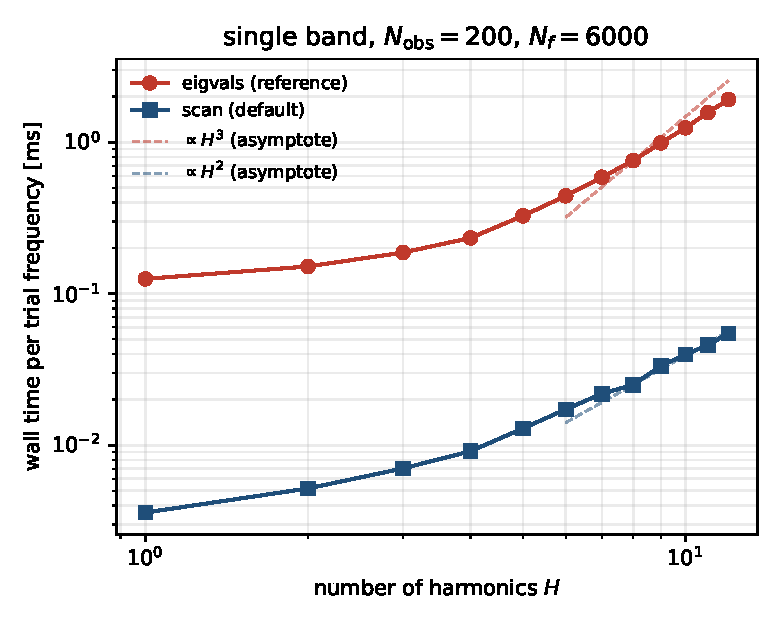
\includegraphics[width=0.5\textwidth]{plots/timing_vs_nharm.pdf}
    \caption{\label{fig:timingnharm} Wall time per trial frequency versus the
            number of harmonics $H$ for the default scan+polish maximiser
            (\texttt{method='scan'}, blue) and the reference polynomial-root
            implementation (\texttt{method='eigvals'}, red), timed on identical
            well-conditioned single-band data ($N_{\rm obs}=200$, $N_f=6000$).
            The default path is a measured factor of $25$--$35$ faster across
            all $H$. At low $H$ both paths are dominated by the shared
            $\bigO(HN_f\log HN_f)$ NFFT summations and rise only mildly with $H$;
            by $H\gtrsim 8$ the per-frequency maximiser takes over, and the
            reference cost steepens toward its $\bigO(H^3)$ root-finding
            asymptote while the scan tracks $\bigO(H^2)$ (dashed segments; the
            measured $8\!\to\!12$ log--log slopes are ${\approx}2.3$ and
            ${\approx}1.9$ respectively).}
\end{figure}

For a fixed number of harmonics $H$, the template periodogram scales as
$\bigO(N_f\log N_f)$. However, for a constant number of trial frequencies $N_f$,
the per-frequency cost grows as $\bigO(H^2)$ on the default scan path
($\bigO(H^3)$ on the reference root-finding path), and computational resources
alone limit $H$ to reasonably small numbers $H\lesssim15$ (see Figure \ref{fig:timingnharm}).

This practical ceiling has a direct bearing on the algorithm's scope of
applicability for box-like signals such as exoplanetary transits and
detached eclipsing binaries.  As we calibrate in
Section~\ref{sec:choiceH}, the canonical analytic trapezoidal-transit and
detached-EB templates considered here have slope (first-derivative)
discontinuities at their ingress/egress corners, which produce a
$\sim 1/n^2$ tail in the Fourier coefficients and require
$H \approx 12$ to reach $95\%$ $L^2$ fidelity and $H \approx 21$ to
reach $99\%$ (Table~\ref{tab:hvsaccuracy}).  FTP therefore \emph{can}
handle transit- and eclipse-shaped signals, but at the upper end of
computationally tractable $H$ values, and at a cost that grows as
$H^2 N_f$ on the default path ($H^3 N_f$ on the reference).  Real
limb-darkened transits are smoother than the
trapezoidal idealisation---they have finite, gently-curved
ingress/egress and consequently Fourier coefficients that decay
faster than the trapezoid's $1/n^2$ tail---so the $H$ requirements
in practice may be lower than Table~\ref{tab:hvsaccuracy} suggests
for a pathological trapezoid.  Nevertheless, for surveys targeting
genuinely box-shaped signals with very sharp ingress/egress
(e.g.\ short-cadence shallow transits or short-duration eclipses),
transit-tailored methods such as the Box Least-Squares periodogram
\citep[BLS,][]{Kovacs_2002}---of which a GPU-accelerated
descendant, CETRA, has recently been described by \citet{Smith_etal_2025}---are
likely to be a more efficient choice than FTP.


\subsection{Choosing the harmonic order \texorpdfstring{$H$}{H}}\label{sec:choiceH}

The harmonic order $H$ is a free parameter of the algorithm.  Two
considerations bound it in practice:  (i) the $L^2$ fidelity of the
$H$-truncated Fourier series as an approximation of the true template
shape, and (ii) the numerical precision of the polynomial-rooting
step at large $H$.

To quantify (i) for representative fixed-shape signals, we evaluated
the cumulative explained-variance fraction
$F(H) = \sum_{n=1}^H (c_n^2 + s_n^2) / \sum_{n=1}^{\infty} (c_n^2 + s_n^2)$
for five canonical analytic templates: an asymmetric exponential
RR\,Lyrae ab pulse (fast rise, slow decline); a skewed sinusoidal
RR\,Lyrae c profile; a trapezoidal planet transit with linear
ingress/egress; a detached eclipsing binary built from two such
trapezoidal eclipses; and a Doppler-beaming$\;+\;$ellipsoidal-modulation
profile (exactly two-harmonic by construction).  Table~\ref{tab:hvsaccuracy}
lists the smallest $H$ that reaches each of the
$F = 0.90, 0.95, 0.99$ thresholds, and Figure~\ref{fig:hvsaccuracy}(a)
shows the full $F(H)$ curves.

\begin{table}
\centering
\caption{\label{tab:hvsaccuracy}
The minimum harmonic order $H_{\min}(F)$ at which the $H$-truncated
Fourier expansion of each canonical template captures the listed
fraction $F$ of its total $L^2$ energy.  The right-hand columns
report the empirical period-recovery rate at peak-to-peak SNR$\,=\,7$
on 30 independent synthetic light curves with
$N_{\rm obs}=100$ irregular samples per trial, comparing the Fast
Template Periodogram at $H = H_{\min}(F{=}0.95)$ with the
single-harmonic Lomb--Scargle-equivalent (FTP at $H{=}1$).
Tabulated values come from the analytic Fourier expansions
described in Section~\ref{sec:choiceH} and from the open-source
reproduction script in the paper repository.}
\begin{tabular}{lcccccc}
\hline
Template & \multicolumn{3}{c}{$H_{\min}(F)$} & \multicolumn{3}{c}{Recovery at SNR\,$=7$} \\
\cline{2-4} \cline{5-7}
& 90\% & 95\% & 99\% & $H$ & FTP & LS-eq. \\
\hline
RR Lyrae ab & 2 & 3 & 8 & $H=3$ & 100\% & 100\% \\
RR Lyrae c & 2 & 2 & 3 & $H=2$ & 100\% & 100\% \\
Planet transit & 6 & 12 & 21 & $H=12$ & 100\% & 47\% \\
Detached EB & 6 & 12 & 21 & $H=12$ & 100\% & 0\% \\
Ellipsoidal + beaming & 2 & 2 & 2 & $H=2$ & 100\% & 0\% \\
\hline
\end{tabular}

\end{table}

The five templates span an order of magnitude in their harmonic
requirements.  At the low end, the ellipsoidal$\;+\;$beaming profile is
exactly band-limited at $H = 2$; the skewed-sinusoid RR\,Lyrae c
reaches $99\%$ at $H = 3$.  The asymmetric-pulse RR\,Lyrae ab
profile reaches $99\%$ at $H = 8$.  At the high end, the trapezoidal
transit and detached-EB templates have slope (first-derivative)
discontinuities at their ingress/egress corners, which gives a
$\sim 1/n^2$ tail in the Fourier coefficients; both require
$H \approx 12$ for $95\%$ fidelity and $H \approx 21$ for $99\%$.
These tabulated values are specific to the $12$ per cent duty cycle
of the analytic trapezoids used here: for a pulse of duty cycle
$\delta$ the Fourier energy extends to harmonics $n \sim 1/\delta$,
so the required harmonic order scales as
$H_{\min}(F) \propto 1/\delta$---a $6$ per cent duty-cycle transit
needs roughly twice the tabulated $H$.
For applications where the underlying signal has sharper features
than these analytic templates (e.g. true limb-darkened transits with
fast cadence), the $99\%$ values may need to be revised upward.

The practical consequence for period detection is shown in
Figure~\ref{fig:hvsaccuracy}(b), which reports the period-recovery
rate of FTP and of the LS-equivalent (FTP at $H{=}1$, i.e. a
single-harmonic sinusoidal template) on synthetic noisy light
curves.  Each light curve consists of $N_{\rm obs} = 100$ samples
drawn uniformly from a $T_{\rm obs} = 100$\,day window with
independent Gaussian noise scaled to the indicated peak-to-peak
SNR; each periodogram is evaluated on the frequency window
$[0.01, 5]$~cyc\,day$^{-1}$ at $10$ samples per peak, and the
period is declared recovered when
$|f_{\rm peak} - f_{\rm true}|/f_{\rm true} < 5\times 10^{-3}$.
Thirty independent trials are run per (template, SNR) cell.
For the smooth, near-sinusoidal RR\,Lyrae profiles the two
estimators agree at all SNRs: at this dense sampling
($N_{\rm obs} = 100$), a single-harmonic template suffices.  (This
conclusion is specific to the dense-sampling regime; in the sparse
regime, where few epochs constrain many free parameters, the
template's shape prior becomes decisive even for these smooth
profiles, as quantified in the sparse-sampling simulation-validation
results of Section~\ref{sec:simval}.)
For the three non-sinusoidal templates (transit, EB,
ellipsoidal$\;+\;$beaming), FTP at $H = H_{95\%}$ recovers the
period in $\geq 29/30$ trials at every SNR tested, while the
LS-equivalent fails completely for EB and
ellipsoidal$\;+\;$beaming ($0/30$ recoveries at all SNRs) and only
partially for the transit template ($4/30$, $14/30$, and $17/30$
at SNR$\,=\,3$, $7$, $15$ respectively).  This is the regime in
which the $H$-truncation matters: harmonics beyond the first are
required to match the underlying signal shape.

For the numerical-precision consideration (ii), we have measured the
maximum periodogram error of the implementation in this paper against
a brute-force evaluation that explicitly maximises $V(\theta,\omega)$
on a dense $\theta_2$ grid with local refinement.  Verified through
$H = 21$ (covering the highest harmonic orders required by
Table~\ref{tab:hvsaccuracy}), the maximum absolute error in
$P(\omega)$ is $\sim 10^{-15}$ with direct summations and
$\sim 10^{-13}$ with the NFFT-based summations.\footnote{Issue \#33 of
the FTP repository at
\url{https://github.com/PrincetonUniversity/FastTemplatePeriodogram/issues/33}
documents the test methodology and the precision floor of
\texttt{numpy.polynomial.polyroots} as used by the implementation.}
The guarantee is one-sided by construction: every candidate root is
projected onto the unit circle and the \emph{true} periodogram is
evaluated there, so the reported power -- a maximum over a finite
candidate set -- can only \emph{under}estimate the true per-frequency
maximum, never overestimate it.  These floors are measured under
homoscedastic measurement errors.  They degrade when a single
observation dominates the total inverse-variance weight budget by a
factor $\gtrsim 10^8$ -- catastrophic cancellation in the weighted
moment sums, which afflicts the fast NFFT-based summations earlier
than direct summations -- and this condition is the practical meaning
of the ``pathological cases'' caveat in the abstract.
The floor is well below any astrophysically relevant amplitude
threshold, so polynomial-rooting error does not limit FTP at the
values of $H$ considered in Table~\ref{tab:hvsaccuracy}.

\begin{figure*}
\centering
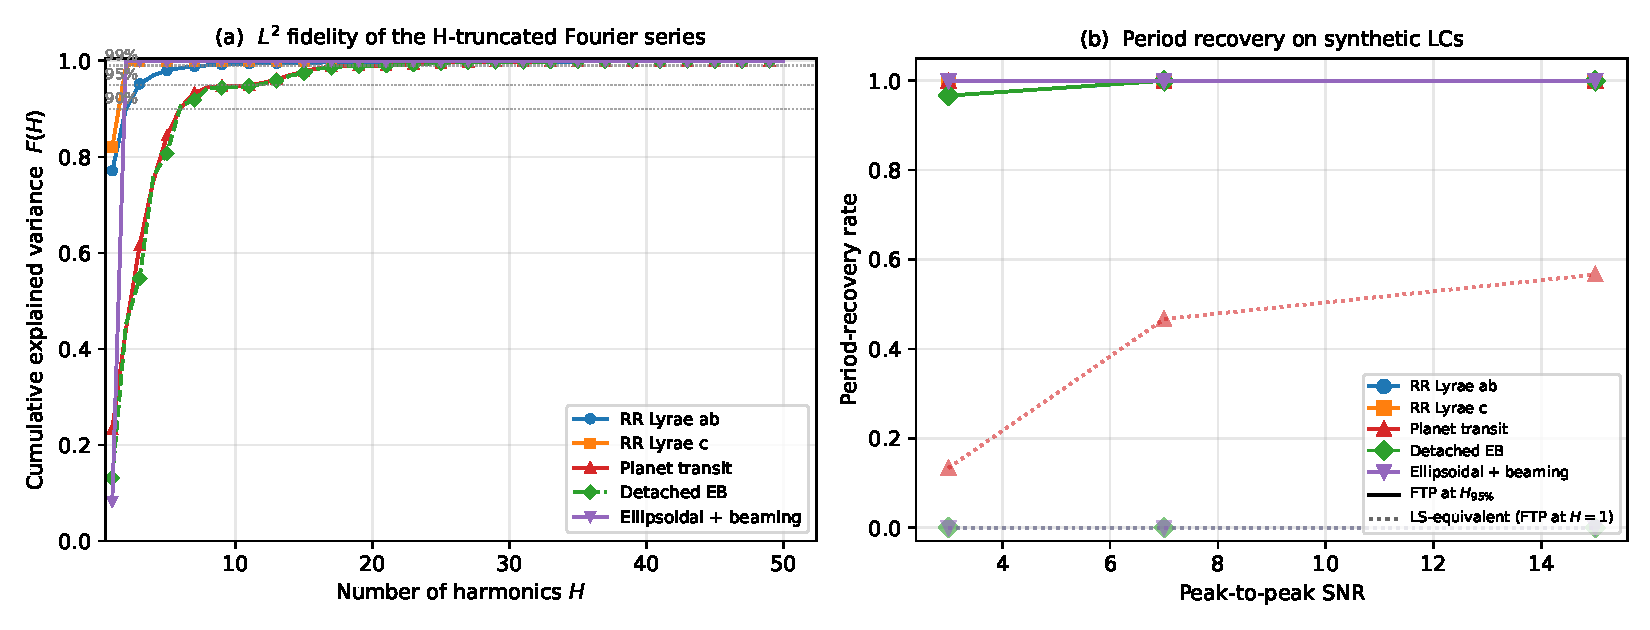
\includegraphics[width=\textwidth]{plots/h_vs_accuracy.pdf}
\caption{\label{fig:hvsaccuracy}
(a) Cumulative $L^2$ explained-variance fraction $F(H)$ of the
$H$-truncated Fourier series as an approximation of each canonical
template.  Horizontal dotted guides mark $F = 0.90, 0.95, 0.99$.
Detached EB and Planet transit have visually overlapping curves
(both driven by sharp ingress/egress discontinuities); the dashed
green line distinguishes the EB.
(b) Empirical period-recovery rate as a function of peak-to-peak
signal-to-noise ratio for densely-sampled $N_{\rm obs} = 100$ synthetic
light curves (30 trials per cell), comparing FTP at
$H = H_{95\%}$ (solid) with the Lomb--Scargle-equivalent FTP at
$H{=}1$ (dotted) for the same five canonical templates.  FTP at
the per-template $H_{95\%}$ recovers the period in $\geq 96\%$ of
trials across the SNR range.  The LS-equivalent agrees with FTP
for the smooth RR\,Lyrae profiles (overlapping solid lines), fails
completely for the EB and ellipsoidal$\;+\;$beaming templates
(flat dotted lines at zero), and recovers only a fraction of
trial transits (red dotted line, climbing from $\sim\!\!13\%$ at
SNR$\,=\,3$ to $\sim\!\!57\%$ at SNR$\,=\,15$).}
\end{figure*}


%\subsubsection{Computational considerations of multi-band extensions}
%Multi-band extensions generally require more computational
%time than the single band case. For the shared-phase multi-band periodogram,
%the scaling becomes $\bigO{KHN_f\log HN_f + K^3H^3N_f}$. The final expression given
%in Equation \ref{eq:condsharedphase} produces a root-finding polynomial that is of order
%$2H(5K - 1)$ for $K > 1$, compared with the order $\sim 6H$ polynomial obtained for
%the $K=1$ case.

%%For the shared phase, amplitude, and offset case, however, the polynomial
%order remains the same as for the single band case, though the time needed to compute
%the polynomial coefficients increases by a factor of $K$.

\section{Implementation}\label{sec:implementation}

\begin{figure*}
    \centering
    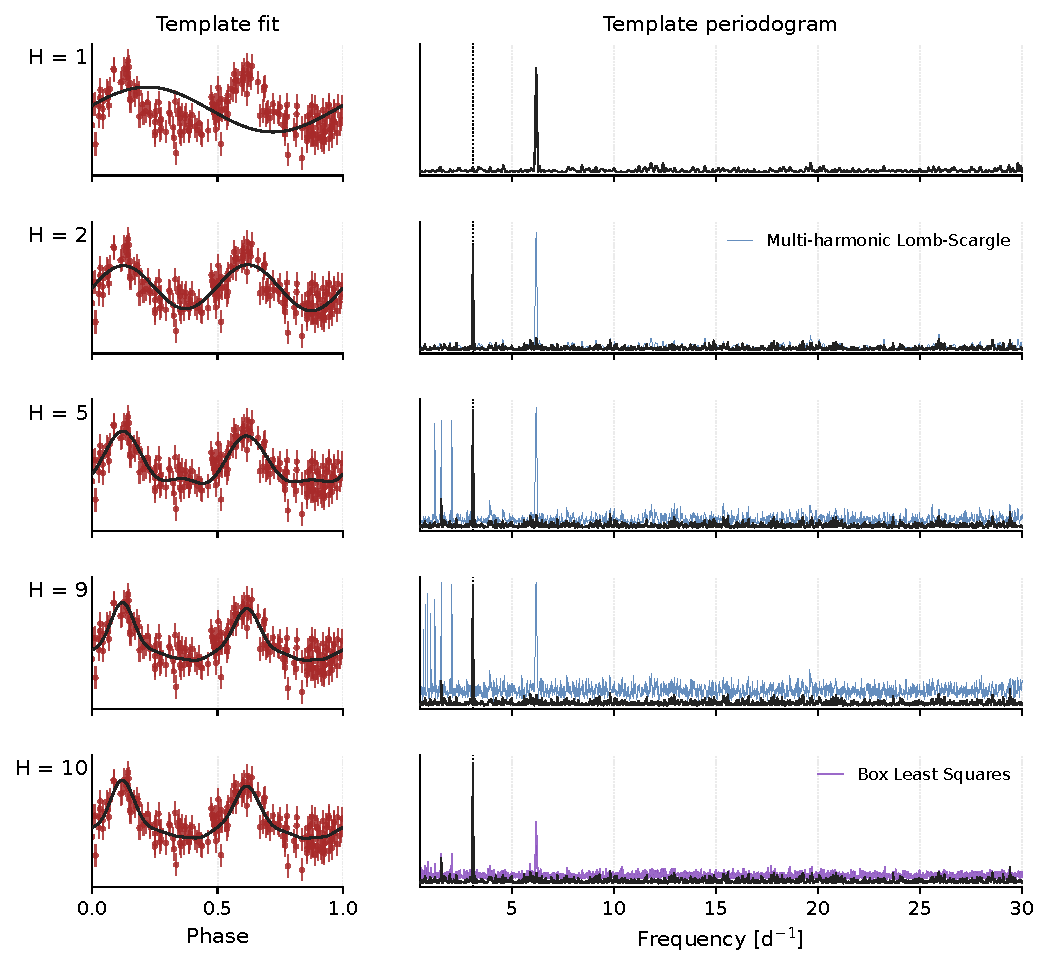
\includegraphics[width=\textwidth]{plots/templates_and_periodograms.pdf}
    \caption{\label{fig:tempsandpdgs} Template periodograms performed on a simulated eclipsing
            binary lightcurve (shown phase-folded in the left-hand plots). The top-most plot
            uses only one harmonic, equivalent to a Lomb-Scargle periodogram. Because the
            simulated eclipsing binary has two minima per orbital cycle, this single-harmonic
            periodogram peaks at twice the true frequency; two or more harmonics are required to
            recover the correct period. Subsequent plots
            use an increasing number of harmonics, which produces a narrower and higher peak
            height around the correct frequency. For comparison, the multi-harmonic extension
            to Lomb-Scargle is plotted in blue, using the same number of harmonics as the FTP.
            The Box Least-Squares \citep{Kovacs_2002} periodogram is shown in the final plot.}
\end{figure*}

An open-source implementation of the Fast Template Periodogram (FTP)
in Python is available.\footnote{\url{https://github.com/PrincetonUniversity/FastTemplatePeriodogram}}
Polynomial algebra is performed using the \texttt{numpy.polynomial} module
\citep{Scipy}. The \texttt{nfft} Python module,
\footnote{\url{https://github.com/jakevdp/nfft}} which provides a Python
implementation of the non-equispaced fast Fourier transform,
is used to compute the necessary sums for a particular time series.

The high-level entry point, \texttt{autopower(samples\_per\_peak=...)},
exposes the trial-frequency grid density as a user parameter:
\texttt{samples\_per\_peak} is the number of trial frequencies that
cover one full-width of a periodogram peak.  Because the peak width
scales roughly as $\delta f_{\mathrm{peak}}\propto 1/H$
(Section \ref{sec:compreqs}), the value of \texttt{samples\_per\_peak}
must scale at least linearly with $H$ to avoid under-sampling the
peaks.  In particular, the shipped default
\texttt{samples\_per\_peak}~$=5$ is a reasonable choice only for
near-sinusoidal ($H=1$) templates: it implies under one trial
frequency per peak at $H=10$, and even a denser
\texttt{samples\_per\_peak}~$=10$ grid -- the conventional
Lomb--Scargle choice -- leaves peaks only about three samples wide in
an empirical inspection at $H=7$, so on the default grid the true
frequency can be missed in favor of a noise peak.  For the sharper templates studied
in Section \ref{sec:choiceH} -- in particular the trapezoidal-transit
and detached-EB shapes, which require $H_{95\%}=12$ in
Table \ref{tab:hvsaccuracy} -- \texttt{samples\_per\_peak}~$\gtrsim 30$
is a more defensible default.  This is the runtime/grid-density
versus peak-recovery tradeoff documented in the open-source
implementation, and users selecting $H$ via Section \ref{sec:choiceH}
should adjust \texttt{samples\_per\_peak} accordingly.

No explicit parallelism is used anywhere in the current implementation,
however certain linear algebra operations in \texttt{Scipy} use OpenMP
via calls to BLAS libraries that have OpenMP enabled.

All timing tests were run on a quad-core 2.6 GHz Intel Core i7 MacBook
Pro laptop (mid-2012 model) with 8GB of 1600 MHz DDR3 memory. The \texttt{Scipy} stack
(version 0.18.1) was compiled with multi-threaded MKL libraries.

\subsection{Comparison with non-linear optimization}

In order to evaluate the accuracy and speed of the template periodogram,
we have included slower alternative solvers within the Python implementation
of the FTP that employ non-linear optimization to find the best fit parameters.

Figure~\ref{fig:tempsandpdgs} shows example periodograms computed for
simulated data, and compares the FTP to the multi-harmonic
Lomb--Scargle (MHLS;
\citealt{Bretthorst+Chi-Cheng_1988,Schwarzenberg-Czerny_1996,Palmer_2009})
and Box Least Squares (BLS; \citealt{Kovacs_2002}) periodograms; the
remaining accuracy and timing comparisons (Figures~\ref{fig:corrwgats}
and~\ref{fig:corrwhighh}) use the same simulated-data prescription.
The simulated data have uniformly random observation times, with
Gaussian-random, homoskedastic, uncorrelated uncertainties.  An
eclipsing binary template, generated by fitting a well-sampled,
high signal-to-noise eclipsing binary in the HATNet dataset
(2MASS\,J02240150+5717241, also known as BD$+56^\circ\,603$) with a
$10$-harmonic truncated Fourier series, is added to the simulated
lightcurves and used as the template for the FTP search.  At the
correct period, the FTP yields a much stronger detection than either
MHLS---which has $2H{+}1$ free parameters and consequently reduces
the signal-to-noise of the periodogram peak relative to a
fixed-shape template---or BLS, which provides only a coarse
box-shaped match to the smooth EB profile.

\subsubsection{Accuracy}

\begin{figure}
    \centering
    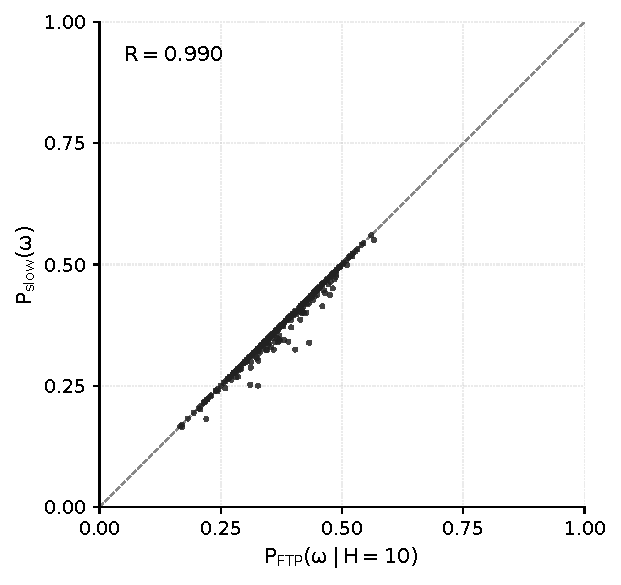
\includegraphics[width=0.5\textwidth]{plots/correlation_with_nonlinopt.pdf}
    \caption{\label{fig:corrwgats} Comparing accuracy between previous methods that rely
            on non-linear optimization at each trial frequency with the fast template periodogram
            described in this paper.  Each point corresponds to one realization of the simulated data
            (an example of which is shown in Figure~\ref{fig:tempsandpdgs}); the axes give the
            \emph{peak} periodogram value $P_{\rm FTP}(\omega\,;\,H{=}10)$ from the FTP and
            $P_{\rm slow}(\omega)$ from the non-linear ``slow'' template fitter, not the
            periodograms themselves.  The annotated $R$ is the Pearson linear-correlation
            coefficient between the two sets of peak values.  The FTP consistently finds more
            optimal template fits than the non-linear solver, which does not guarantee convergence
            to a globally optimal solution; in realizations where the slow fitter is trapped in a
            local $V$-minimum, it reports a higher residual $V$ and therefore a lower peak
            $P_{\rm slow}$ than the FTP, producing the points below the diagonal at low
            $P_{\rm FTP}$.}
\end{figure}

\begin{figure*}
    \centering
    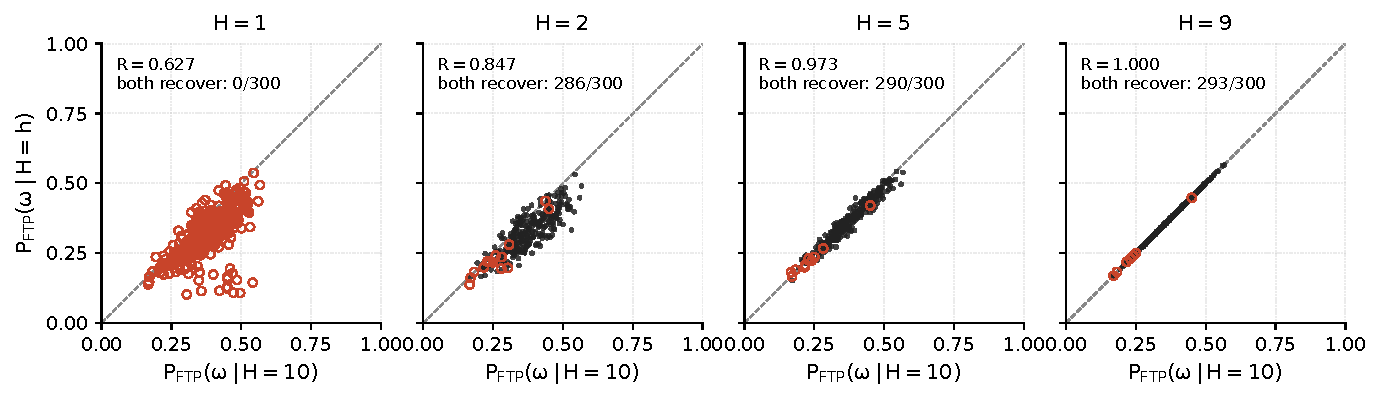
\includegraphics[width=\textwidth]{plots/correlation_with_large_H.pdf}
    \caption{\label{fig:corrwhighh} Similar to Figure~\ref{fig:corrwgats}.  Here we compare the
            template periodogram calculated with $H = 10$ harmonics to the template periodogram
            using a smaller number of harmonics $H < 10$.  Each point is the \emph{peak} periodogram
            value from one realization; $R$ is again the Pearson linear-correlation coefficient
            between the two sets of peak values.  The template and data prescription match those of
            Figure~\ref{fig:tempsandpdgs}.}
\end{figure*}

For weak signals or signals folded at the incorrect trial period, the
$V$ surface in $\theta_2$ admits up to $6H{-}2$ stationary points with
$YM \neq 0$ (the degree bound of the polynomial in
Equation~\ref{eq:finalpoly}; up to $2H$ further stationary points
where $YM = 0$ are zero-power minima, factored out of
Equation~\ref{eq:finalpoly}), so
non-linear optimization algorithms can fail to find the global minimum
and instead lock onto one of the spurious local extrema.  The FTP
sidesteps this entirely by enumerating all roots of
Equation~\ref{eq:finalpoly} and choosing the one that yields the
largest $P(\omega)$, so it recovers the optimal solution even when
the signal is weak or absent.

Figure \ref{fig:corrwgats} illustrates the accuracy improvement with FTP.
Many solutions found via non-linear optimization are significantly suboptimal
compared to the solutions found by the FTP.

Figure \ref{fig:corrwhighh} compares FTP results obtained using the full template
$(H=10)$ with those obtained using smaller numbers of harmonics. The left-most
plot compares the $H=1$ case (weighted Lomb-Scargle), which, as also demonstrated
in Figure \ref{fig:tempsandpdgs}, illustrates the advantage of the template
periodogram for known, non-sinusoidal signal shapes.


\subsubsection{Computation time}

\begin{figure*}
    \centering
    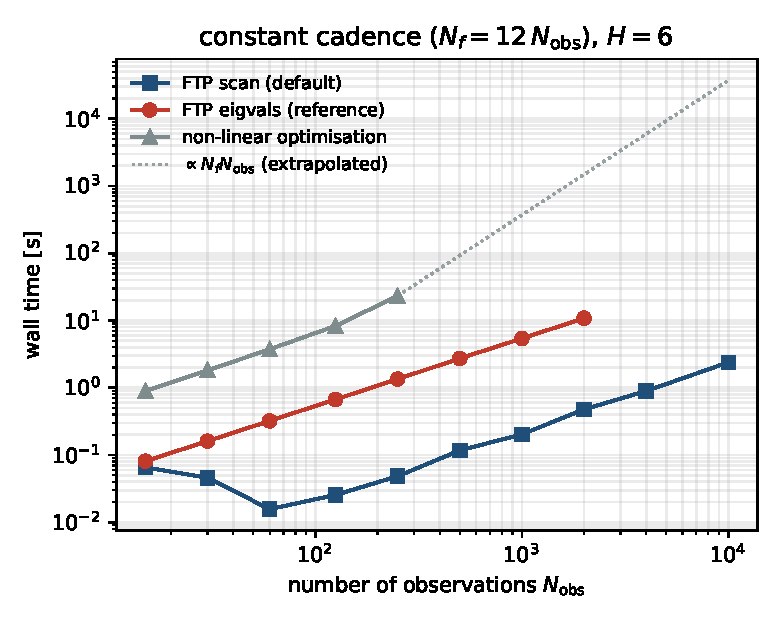
\includegraphics[width=0.45\textwidth]{plots/timing_vs_ndata.pdf}
    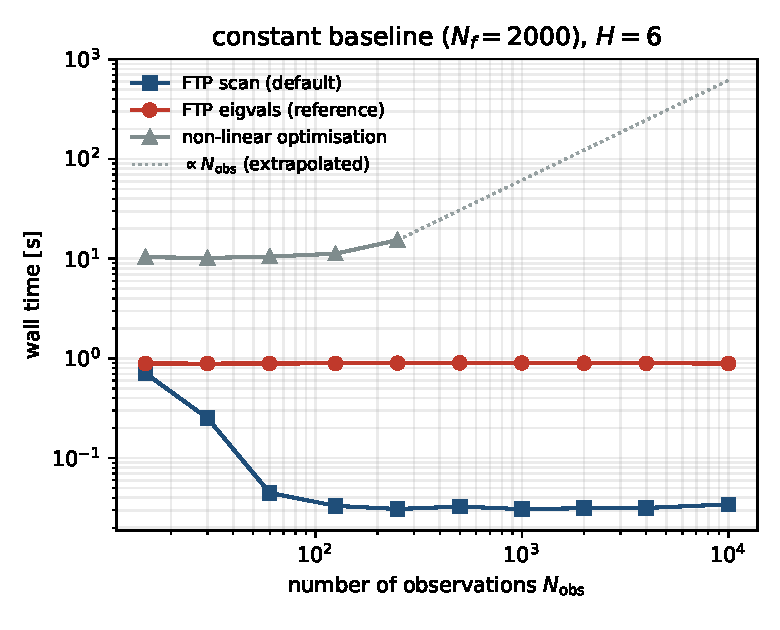
\includegraphics[width=0.45\textwidth]{plots/timing_vs_ndata_const_freq.pdf}
    \caption{\label{fig:timingndata} Computation time of the FTP (default scan
             path, \texttt{method='scan'}, blue; reference root-finding path,
             \texttt{method='eigvals'}, red) compared with full non-linear
             optimization at each trial frequency (grey; $10$ random phase
             restarts per frequency). \emph{Left}: timing for
             the case when $N_f = 12 N_{\rm obs}$, i.e. the cadence of the
             observations is constant. \emph{Right}: timing for the case when
             $N_f$ is fixed, i.e. the baseline of the observations is constant.
             Non-linear optimization scales as $\bigO(N_f N_{\rm obs})$ (dotted
             extrapolation beyond the largest tractable point) while the FTP
             scales as $\bigO(HN_f\log HN_f + N_fH^2)$ on its default path
             ($N_fH^2 \to N_fH^3$ on the reference path), independent of
             $N_{\rm obs}$; $H$ is the number of harmonics needed to approximate
             the template. In the constant-baseline panel the scan cost rises
             toward the reference at the sparsest $N_{\rm obs}$, where the
             rank-deficient sampling triggers the exact-root fallback.}

\end{figure*}

On its default scan path the FTP scales asymptotically as $\bigO(N_fH\log N_fH)$ with respect to the number of trial frequencies,
$N_f$, and as $\bigO(N_fH^2)$ with respect to the number of harmonics in which the template is expanded, $H$
(the reference root-finding path replaces $N_fH^2$ by $N_fH^3$).
For a given resolving power, however, there is an additional factor of $H$ in each of these terms due to the
number of trial frequencies necessary to resolve a periodogram peak being proportional to $H$.
For all reasonable $N_f$ the computation time is dominated by computing the polynomial coefficients and the
per-frequency phase maximisation, both of which scale linearly in $N_f$.

The number of trial frequencies needed for finding astrophysical signals in a typical photometric time series is

\begin{equation}
    N_f = 1.75 \times 10^6 \left(\frac{H}{1}\right)\left(\frac{{\rm baseline}}{10~{\rm yrs}}\right)\left(\frac{\alpha}{5}\right)\left(\frac{15~{\rm mins}}{P_{\rm min}}\right)
\end{equation}

\noindent where $\alpha$ represents the ``oversampling factor,'' $\Delta f_{\rm peak} / \Delta f$, where $\Delta f_{\rm peak} \sim 1/{\rm baseline}$ is
the typical width of a peak in the periodogram and $\Delta f$ is the frequency spacing of the periodogram.

The per-frequency phase maximisation dominates the run time in this regime, which is precisely why replacing the
reference polynomial root-finding with the scan+polish maximiser---now the default in the accompanying
implementation---is worthwhile. On well-conditioned single-band data the default path is a measured factor of
$25$--$35$ faster than the reference Python implementation (\texttt{method='eigvals'}), and this factor is
grid-stable in $N_f$: at $H=8$ we measure ${\approx}32\times$, ${\approx}29\times$ and ${\approx}28\times$ at $N_f=2{,}000$, $8{,}000$ and
$20{,}000$ respectively (Figure~\ref{fig:timingnharm}).

Figure \ref{fig:timingndata} compares the timing of the FTP (default scan path) with that of previous methods that
employ non-linear optimization at each trial frequency. Over the range where the non-linear solver remains tractable,
the default FTP is already a measured factor of ${\sim}14$--$15$ faster at the sparsest, most rank-deficient test case
($15$ datapoints, where the scan itself falls back to the exact root path) and ${\sim}480$--$500$ faster by
$N_{\rm obs}=250$, in both the constant-cadence ($N_f\propto N_{\rm obs}$) and constant-baseline ($N_f$ fixed)
regimes. Because non-linear optimization scales as $\bigO(N_f N_{\rm obs})$ while the FTP's per-frequency cost is
independent of $N_{\rm obs}$, this advantage grows without bound as $N_{\rm obs}$ increases (dotted extrapolation in
Figure~\ref{fig:timingndata}).


% The 10^120 figure comes from the fact that for a test case (Ndata = 500, H = 5, Nf = 14917),
% The fast summations take 8.905e-05 s / freq and the autopower() method takes 2.561e-03 s / freq.
% The fast summation step scales as Nf \log Nf while the rest of the steps scale as Nf (for constant H)
% So we have that
%    t_sums/freq  = alpha * log10(Nf)
%    t_other/freq = beta
%
% t_total(Nf0) = 2.561e-03 = t_sums(Nf0) + t_other(Nf0) = alpha * log10(Nf0) + beta
% and t_sums(Nf0) = 8.905e-05 = alpha * log10(Nf0)
% so alpha = 8.905e-05 / (log10(14917)) = 2.134e-05
% and beta = (2.64E-3 - 8.905e-05) = 2.55e-3
% beta/alpha = 120

% f_sums = t_sums(Nf) / t_total(Nf) = alpha * log10(Nf) / (beta + alpha * log10(Nf))
% f_sums ( beta + alpha log10(Nf)) = alpha * log10(Nf)
% alpha * ( 1 - f_sums) * log10(Nf) = f_sums * beta
% log10(Nf) = (beta / alpha) * (f_sums / (1 - f_sums))
% Nf = 10 ^ ((beta / alpha) * (f_sums / (1 - f_sums)))
%
% Nf = 10 ^ (120 * (f_sums / (1 - f_sums)))
% when f_sums = 0.5 (the point at which the summations dominate the computation time)
% Nf = 10^120!!


\subsection{Significance and false-alarm calibration}
\label{sec:fap}

\begin{figure*}
    \centering
    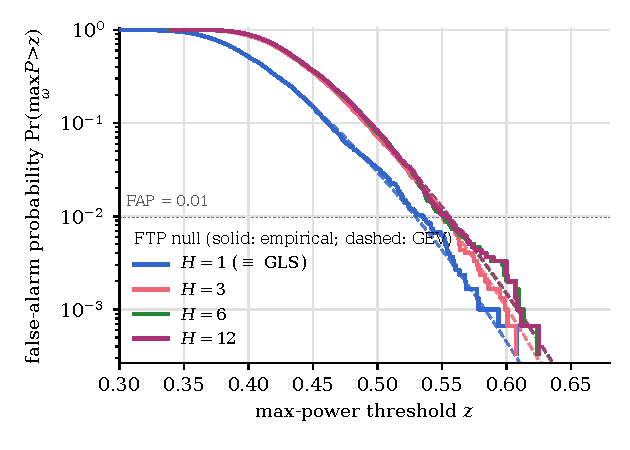
\includegraphics[width=0.45\textwidth]{plots/fap_vs_threshold.pdf}
    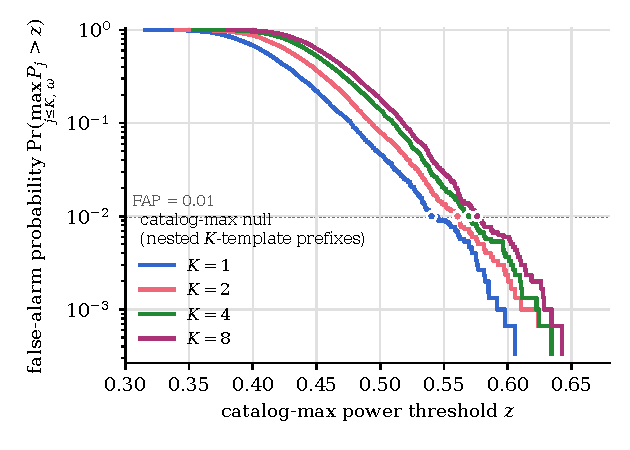
\includegraphics[width=0.45\textwidth]{plots/nullmax_vs_K.pdf}
    \caption{\label{fig:fap} Measured pure-noise null of the maximum
             periodogram power ($3000$ realizations; single band,
             $N_{\rm obs}=40$, three-year seasonal cadence, homoscedastic
             $\sigma \approx 0.010$\,mag; $10^4$ trial frequencies on
             $[1,5]$\,cyc\,day$^{-1}$).  \emph{Left}: false-alarm probability
             versus max-power threshold for the FTP at
             $H \in \{1, 3, 6, 12\}$ (solid: empirical survival function;
             dashed: generalised-extreme-value fit).  The $H{=}1$ curve is
             identical to GLS; the inflation from the non-linear phase family
             appears at $H \geq 3$ and is nearly saturated there.
             \emph{Right}: null of the catalog-max statistic for nested
             $K$-template prefixes of a single $K{=}8$ vocabulary; markers
             show the empirical ${\rm FAP}=0.01$ thresholds, which grow from
             $0.540$ ($K{=}1$) to $0.576$ ($K{=}8$) -- the pure extra-trials
             cost of a larger vocabulary.}
\end{figure*}

At a fixed trial frequency the template periodogram is not the score of a
linear model of fixed dimension: the model
$\hat{y} = \theta_1\Mshft + \theta_3$ has only three free parameters, but the
phase $\theta_2$ enters non-linearly, and the reported power is a maximum over
the up-to-$(6H{-}2)$ stationary phases of Equation~\ref{eq:finalpoly}.  The
classical per-frequency null for linear periodograms (an incomplete-beta /
$\chi^2$ law with the model's degrees of freedom) therefore does not apply
directly; the natural framework is the extreme-value treatment of
\cite{Baluev_2008}, with an \emph{effective} number of degrees of freedom
inflated relative to the single-sinusoid case.  Rather than derive a bound,
we measure the null directly: $3000$ pure-noise light curves at a
production-like cadence (single band, $N_{\rm obs}=40$, three-year baseline
with $270$-day observing seasons, homoscedastic $\sigma \approx 0.010$\,mag),
searched over $10^4$ trial frequencies on $[1,5]$\,cyc\,day$^{-1}$ with
RR\,Lyrae-medoid templates truncated at order $H$, alongside a floating-mean
(generalised) Lomb--Scargle baseline \citep[GLS;][]{Zechmeister+Kurster_2009}.
Two facts summarise the measurement (Figure~\ref{fig:fap}, left).  First, at
$H=1$ the FTP \emph{is} the GLS: the per-realization maximum powers agree to
a maximum absolute difference of $1.2\times10^{-9}$ over all $3000$
realizations, as they must -- a single-harmonic template spans the same
linear space as a floating-mean sinusoid.  Second, the inflation from
the non-linear phase family is modest and saturates almost immediately: the
mean null maximum rises from $0.407$ at $H=1$ to $0.440$ at $H=3$, then
$0.442$ ($H=6$) and $0.443$ ($H=12$), and the empirical ${\rm FAP}=0.01$
threshold rises from $0.535$ ($H=1$) to $0.551$, $0.551$, and $0.553$ at
$H=3$, $6$, and $12$.  An $H=12$ template therefore costs less than $+0.02$
in detection threshold at the calibrated ${\rm FAP}=0.01$ relative to
Lomb--Scargle -- far below the cost of the $2H{+}1 = 25$ free coefficients
of a multi-harmonic fit of the same order -- because the fixed template
shape confines the maximisation to a one-parameter curve of phase shifts
inside the $(2H{+}1)$-dimensional harmonic space.
Generalised-extreme-value fits (dashed curves in Figure~\ref{fig:fap})
describe the empirical curves well and extend the thresholds beyond the
Monte-Carlo resolution.

The statistic being calibrated is the normalised power of
Equation~\ref{eq:lsp}, $P = (V_0 - V)/V_0$ -- equivalently
$1 - \chi^2/\chi^2_0$, since $\chi^2 = W V$ (Section~\ref{sec:max-likelihood})
-- which is confined to $[0,1]$: $V \geq 0$ gives the upper bound, and the
constant-only null model is nested in the template model, so $V \leq V_0$.
In the multi-band hierarchy of Appendix~\ref{sec:shphmult} the reference
variance $V_0$ differs by sharing mode (Table~\ref{tab:sharingmodes}): the three modes that
retain a per-band offset (\texttt{independent}, \texttt{shared\_phase},
\texttt{floating\_offsets}) measure power against the per-band-centred
variance $\sum_k \Wtk YY^{(k)}$, whose null model is a separate constant per
band, whereas the fully shared \texttt{sesar} mode measures power against the
global weighted variance of the data after subtracting its fixed per-band
offsets $\lk$, whose null model is a single global constant.  Null
distributions, and therefore detection thresholds, calibrated for one mode
do not transfer to another, even on identical data.

When a vocabulary of $K$ templates is searched and the maximum power over the
vocabulary is reported (the catalog-max statistic
$\max_{j \leq K}\max_\omega P_j(\omega)$), the null acquires a $K$-dependence:
an extra-trials cost.  A Bonferroni bound,
${\rm FAP}_K(z) \leq K\,{\rm FAP}_1(z)$, is always valid but conservative,
because the per-template statistics are computed on the same data and the
templates share their low-order harmonics.  The measured null
(Figure~\ref{fig:fap}, right; nested prefixes of a single $K{=}8$
partitioning-around-medoids vocabulary built from the \citealt{Sesar_etal_2010}
RR\,Lyrae library) quantifies both statements: the mean null maximum grows
from $0.422$ ($K{=}1$) to $0.467$ ($K{=}8$) and the ${\rm FAP}=0.01$ threshold
from $0.540$ to $0.576$, while at that measured $K{=}8$ threshold a single
template has ${\rm FAP} = 0.0030$, so the Bonferroni estimate
($8 \times 0.0030 = 0.024$) overstates the measured $0.010$ by a factor
$2.4$.  This extra-trials cost is a shift of the null in power units and
is not directly commensurate with a recovery \emph{rate}; the appropriate
yardstick for the small, non-monotonic wobble of period-recovery rate with
vocabulary size in the sparse-sampling recovery simulations
(Section~\ref{sec:simval-ksweep}; RRab-dominated
universe, $768$ pooled sources per cell) is the binomial sampling
uncertainty: the pooled rate at
$K = 1$, $2$, $4$, $8$ is $0.716$, $0.715$, $0.738$, $0.741$, with Wilson
$95\%$ intervals $[0.683, 0.747]$, $[0.682, 0.746]$, $[0.706, 0.768]$,
$[0.709, 0.771]$ -- a non-monotone range of $0.026$ with mutually
overlapping intervals, and therefore not
evidence of a vocabulary-quality effect at this sampling.

Two caveats bound this calibration.  First, the null is calibrated at a
single configuration -- one band, $N_{\rm obs}=40$, this cadence and grid --
and the thresholds shift with the number of observations, the band
structure, and the grid density, so they do not transfer to other survey
configurations without recalibration.  Second,
the null's $K$-axis isolates the pure extra-trials cost by nesting prefixes
of one fixed $K{=}8$ vocabulary, whereas the production $K$-sweep rebuilds an
independent vocabulary at each $K$ -- the template identities themselves
change with $K$ -- an effect bounded by the measured ${\sim}0.025$ spread of
the per-template null-max means across the eight vocabulary templates.
Finally, this section calibrates \emph{significance} only: the completeness
and purity of template-based detection at a controlled false-alarm rate are
survey-specific questions deferred to follow-up work.


\section{Template vocabularies for heterogeneous signal classes}
\label{sec:vocab}

The preceding sections assume a single, \emph{a priori} known template.
Real signal classes are heterogeneous -- RR\,Lyrae alone span
fundamental-mode (ab) and first-overtone (c) morphologies -- so a blind
search must instead carry a small \emph{vocabulary} of $K$ templates and
report the per-frequency maximum power over the set (the catalog-max
statistic whose null is calibrated in Section~\ref{sec:fap}).  The
computational cost is $K$ times the single-template cost, so the
vocabulary must be small and representative.  This section describes how
the accompanying implementation constructs such vocabularies from a
library of empirical light-curve shapes; Section~\ref{sec:simval}
validates the resulting searches on simulated sparse multi-band surveys.

\emph{Shape space and invariances.}
Every library shape is stored as a truncated Fourier series
(Equation~\ref{eq:templateFourier}) with no constant term, rescaled at
construction to unit Fourier energy, $\sum_{k=1}^{H}(c_k^2+s_k^2)=1$.
Vertical offset and overall scale -- the parameters $\theta_3$ and
$\theta_1$ that the periodogram itself fits per source -- are therefore
quotiented out before any shape comparison.  Phase is removed by the
dissimilarity itself, the orbit-minimized $L^2$ distance
\begin{equation}\label{eq:orbitdist}
    d^2(f, g) \;=\; \min_{\Delta\in[0,1)}
    \bigl\Vert f - g(\cdot - \Delta)\bigr\Vert^2
    \;=\; 1 - \max_{\Delta} {\rm CC}(\Delta),
\end{equation}
where ${\rm CC}(\Delta)$ is the circular cross-correlation of the two
harmonic-coefficient sequences ($w_k = z^{(f)}_k \overline{z^{(g)}_k}$
with $z_k = c_k - i s_k$) and the norm is scaled so that a unit-energy
shape has $\Vert f \Vert = 1$.  The phase maximization is solved exactly
per pair: ${\rm CC}$ is a degree-$H$ trigonometric polynomial, evaluated
on an alias-free oversampled FFT grid (size $\geq 8H+1$, rounded up to a
power of two), after which every cyclic local maximum is polished by
Newton iterations on the closed-form ${\rm CC}'/{\rm CC}''$; the reported
distance is machine-precision, not grid-limited.  Reflections
(time-reversals) are deliberately \emph{not} identified: the
fast-rise/slow-decline asymmetry of an RRab light curve is a physical,
discriminating feature, so a mirrored shape is a distinct template.

\emph{Unsupervised selection (PAM $k$-medoids).}
Given the symmetric matrix of pairwise orbit distances, the default
selector is classical partitioning around medoids
\citep{Kaufman+Rousseeuw_1990} on the objective
$\sum_i \min_{m} d(f_i, f_m)$ (unsquared distances): a greedy
\textsc{build} seeding followed by \textsc{swap} descent, which applies
the single best strictly cost-reducing (medoid, non-medoid) exchange
until none remains, with ten restarts (the deterministic \textsc{build}
plus nine seeded random size-$K$ subsets) and the lowest-cost solution
kept.  Medoids are actual library members, so every vocabulary template
is a physical light-curve shape rather than a cluster average.  The
vocabulary size $K$ is an input, chosen externally by the
recovery-versus-$K$ experiments of Section~\ref{sec:simval}.  A
fixed-chart alternative distance built on the classical Fourier
invariants $R_{k1} = A_k/A_1$ and $\phi_{k1} = \phi_k - k\phi_1$
\citep{Simon+Lee_1981} is retained purely as a validation diagnostic
(agreement of nearest-medoid assignments with the orbit metric); it
degenerates when the first-harmonic amplitude vanishes, so the orbit
distance is the reference.

\emph{Recovery-driven selection (greedy set cover).}
The second selector optimizes the search objective directly.  A seeded
population of synthetic multi-band light curves is simulated once from
the truth shapes and target cadence (Section~\ref{sec:simval}) and
frozen; for every library template the \emph{standalone} mask of sources
whose period that single template recovers is precomputed; and templates
are then forward-selected by set cover -- each step adds the template
that recovers the most not-yet-recovered sources, with ties broken
deterministically -- stopping at $K$ templates, at zero marginal gain, or
at full coverage.  Because the catalog statistic is a per-frequency
maximum over the set, the union of standalone masks is used only as the
selection signal; the returned figure of merit re-scores the chosen
$K$-template catalog end-to-end.  If coverage saturates before $K$
selections, the set is padded to exactly $K$ by farthest-point selection
under the orbit distance (the saturation point is itself the empirical
knee).  An optional pre-filter restricts the candidate universe to the
$M \geq K$ PAM medoids of the full library, capping the standalone-mask
precompute; recovery-versus-$K$ curves built on such a pool are lower
bounds on the all-library curves.  To keep the selection honest, the
selection population is always simulated on a random split disjoint from
any population used for evaluation.

\emph{Template libraries.}
Two empirical RR\,Lyrae libraries are used.  The \citet{Sesar_etal_2010}
SDSS Stripe~82 templates contribute one library shape per (star, band)
pair; the $g,r$ subset used here comprises $98$ shapes, nearly all RRab.
The \citet{Baeza-Villagra_etal_2025} DECam $griz$ templates contribute
$136$ RRab and $144$ RRc stars; their $g,r$ subset comprises $560$
shapes and is deliberately more morphologically diverse.  Library curves
are ingested by resampling each published template onto a uniform phase
grid and taking the real FFT truncated at a common harmonic order
($H = 8$ throughout this section and the next), dropping the constant
term and renormalizing to unit energy; libraries supplied at a different
order are truncated or zero-padded to the common $H$ and renormalized.

\section{Validation on simulated sparse multi-band surveys}
\label{sec:simval}

\subsection{Simulation harness and comparison methods}
\label{sec:simval-harness}

Each experiment freezes a seeded population of $256$ synthetic two-band
($g,r$) light curves per seed, with three seeds pooled for the headline
cells ($768$ sources per cell).  Every source draws a truth shape
uniformly from the truth library, a period $P = 1/f$ with $f$ uniform on
the search band, and a random phase; the unit-energy shape is scaled by
$0.5$\,mag (an rms amplitude of $0.5/\sqrt{2} \approx 0.35$\,mag, shared
across bands) around a mean magnitude of $15$, and observed with
heteroscedastic Gaussian noise
$\sigma(m) = 0.01 + 0.005\,e^{\,m-20}$
($\approx 0.010$\,mag at the simulated magnitudes).  Epochs are drawn
independently per band, uniformly within $270$-day yearly observing
seasons across a three-year ($T = 1095.75$\,d) baseline; a $60$-epoch-%
per-band master cadence is downsampled to
$N \in \{4, 8, 12, 16, 24, 40\}$ epochs per band, so all epoch counts
score the \emph{identical} sources and method contrasts are paired.
A period is recovered when $|P_{\rm rec}-P_{\rm true}|/P_{\rm true} <
0.01$, with \emph{no} credit for harmonic or window aliases (an
alias-resolved re-scoring is given in Appendix~\ref{app:aliases});
uncertainties are Wilson $95\%$ intervals on pooled counts and paired
method contrasts are exact McNemar tests \emph{on the same sources}.
All methods reduce to $P_{\rm rec} = 1/{\rm argmax}$ over the identical
explicit grid: $10^4$ trial frequencies on $[1, 5]$\,cyc\,day$^{-1}$
(RR\,Lyrae periods $0.2$--$1$\,d), i.e.\ a grid spacing
$\Delta f = 4.0\times10^{-4}$\,cyc\,day$^{-1}$ or $2.28$ grid points per
Rayleigh width $1/T$ -- every run records $\Delta f$ and this
points-per-Rayleigh figure, and a hard guard rejects configurations with
fewer than two points per Rayleigh width.

The comparison methods bracket the multi-band model space.  The
generalised Lomb--Scargle baseline
\citep[GLS;][]{Zechmeister+Kurster_2009} fits one shared sinusoid plus
per-band offsets -- the $(N_{\rm base}, N_{\rm band}) = (1, 0)$ corner of
the \citet{Vanderplas+Ivezic_2015} multi-band family -- while the
multi-band LS baseline (MBLS) gives each band its own floating-mean
sinusoid sharing only the period, their $(0, 1)$ corner.  The
multi-harmonic Lomb--Scargle
\citep[MHLS;][]{Schwarzenberg-Czerny_1996} is the free-shape reference:
a shared Fourier series of requested order $H = 8$ plus per-band
offsets, with the order capped per light curve at
$H_{\rm eff} = \max\{1, \min[H, \lfloor(N_{\rm obs} - 2 n_{\rm bands})/4\rfloor]\}$
so that the design never reaches rank deficiency (an uncapped $H=8$
design has $p \geq N_{\rm obs}$ columns at sparse $N$ and interpolates
every point, making the argmax meaningless); at $4$ epochs per band the
cap forces $H_{\rm eff} = 1$ and MHLS is verifiably identical to GLS.
The conditional-entropy statistic \citep[CE;][]{Graham_etal_2013b}
represents binned folding methods: each band min--max normalised, bands
merged, and $H(m|\phi)$ minimised over a $10\times5$
(phase\,$\times$\,magnitude) histogram.  The FTP is run in catalog mode
(\texttt{floating\_offsets}, $H = 8$) with $K = 2$ vocabularies built by
both selectors of Section~\ref{sec:vocab} from the same library that
generates the truth shapes (robustness to that assumption is tested
below).

\subsection{Recovery versus epochs per band}
\label{sec:simval-nsweep}

\begin{figure}
    \centering
    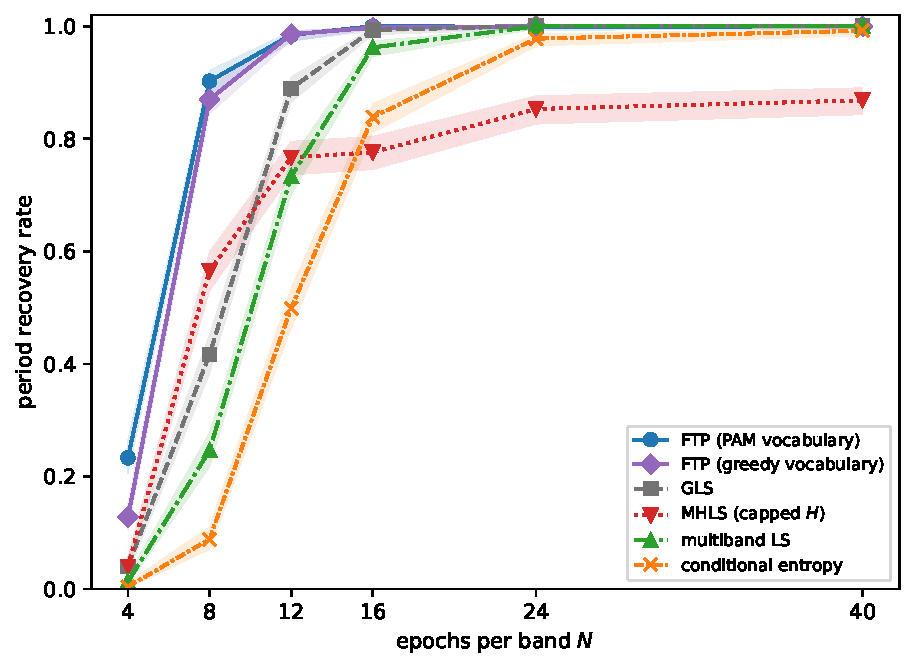
\includegraphics[width=\columnwidth]{plots/recovery_vs_nepochs_sesar.pdf}
    \caption{\label{fig:nsweep} Period-recovery rate versus epochs per
             band on the RRab-dominated \citet{Sesar_etal_2010} universe
             ($768$ pooled sources per cell; bands are Wilson $95\%$
             intervals on pooled counts; vocabulary size $K = 2$).  The
             template vocabulary dominates every free-shape and binned
             method in the sparse regime ($N \lesssim 12$ epochs per
             band) and converges with the sinusoidal baselines once the
             data constrain their models ($N \gtrsim 16$).  MHLS
             plateaus below $0.9$ because its extra freedom locks onto
             harmonic aliases (Appendix~\ref{app:aliases}).  Absolute
             rates in the sparse cells are lower bounds at this grid
             density (see the grid-resolution caveat in the text).}
\end{figure}

Figure~\ref{fig:nsweep} shows the headline result.  At $8$ epochs per
band the PAM-vocabulary FTP recovers $0.902$ $[0.879, 0.921]$ of
sources versus $0.417$ $[0.382, 0.452]$ for GLS -- a paired contrast of
$392$ sources recovered only by the FTP against $19$ only by GLS
(McNemar $p \approx 10^{-91}$) -- and $0.246$ for MBLS, $0.089$ for CE.
At the sparsest cell ($N = 4$, where the MHLS cap makes every
sinusoidal baseline identical to GLS) the FTP still recovers $0.233$
$[0.205, 0.264]$ versus $0.040$ $[0.029, 0.057]$ ($169$ vs.\ $21$
discordant sources, $p \approx 10^{-29}$).  By $N = 16$ the sinusoidal
and template methods have all converged to ${\gtrsim}0.96$ (FTP vs.\
GLS: $5$ vs.\ $0$ discordant, $p = 0.06$), the binned CE statistic
converges near $N = 40$ ($80$ merged points against $50$ histogram
cells), and MHLS alone plateaus at $0.868$ $[0.843, 0.891]$: its
$2H$ free coefficients happily fit the data at half or a third of the
true frequency, and Appendix~\ref{app:aliases} shows its residual
failures are indeed dominated by $2P$/$3P$ harmonic aliases rather than
noise.  The two vocabulary selectors agree closely on this
shape-matched universe, with a small but significant PAM advantage in
the sparsest cells ($124$ vs.\ $43$ discordant at $N = 4$,
$p \approx 3\times10^{-10}$); the greedy selector's value appears on
the mismatched-library arm below.

% ===================================================================
% GRID-RESOLUTION CAVEAT -- single point of update.  When the WP
% B8-closure dense-grid (or peak-refinement) rerun lands, update the
% numbers in THIS paragraph only (and the one caption cross-reference
% in Figure~\ref{fig:nsweep}).
% ===================================================================
\emph{Grid-resolution caveat.}
The absolute sparse-regime rates above are \emph{lower bounds at the
stated $10^4$-frequency production grid} for the $H = 8$ and binned
methods.  A multi-harmonic peak has width ${\sim}\,{\rm Rayleigh}/H$, so
the production grid places only ${\approx}\,0.29$ points per $H = 8$
peak width.  A paired convergence check re-scoring the identical seed-0
sources on a $2\times10^4$-frequency grid ($4.56$ points per Rayleigh
width) finds $8$ of $30$ (method, $N$) cells significantly changed
(exact McNemar, $p < 0.05$), \emph{all} gaining at the denser grid:
MHLS gains most (up to $+0.17$ at $N = 12$), the FTP gains in one cell
($N = 8$: $0.926 \rightarrow 0.973$, $+17/-5$ discordant, $p = 0.017$),
CE in two, MBLS in one, and GLS in none (all $p \geq 0.13$).  The
method \emph{ordering} is unaffected: the FTP$-$GLS recovery margin is
equal or wider on the denser grid ($0.20 \rightarrow 0.25$ at $N = 4$;
$0.539$ on both grids at $N = 8$), so the FTP-versus-GLS contrasts
quoted here are conservative.  A dense-grid closure rerun will finalize
the absolute sparse-cell rates; every absolute rate in this section is
quoted ``at the $10^4$-frequency production grid.''

\subsection{Recovery versus vocabulary size}
\label{sec:simval-ksweep}

\begin{figure*}
    \centering
    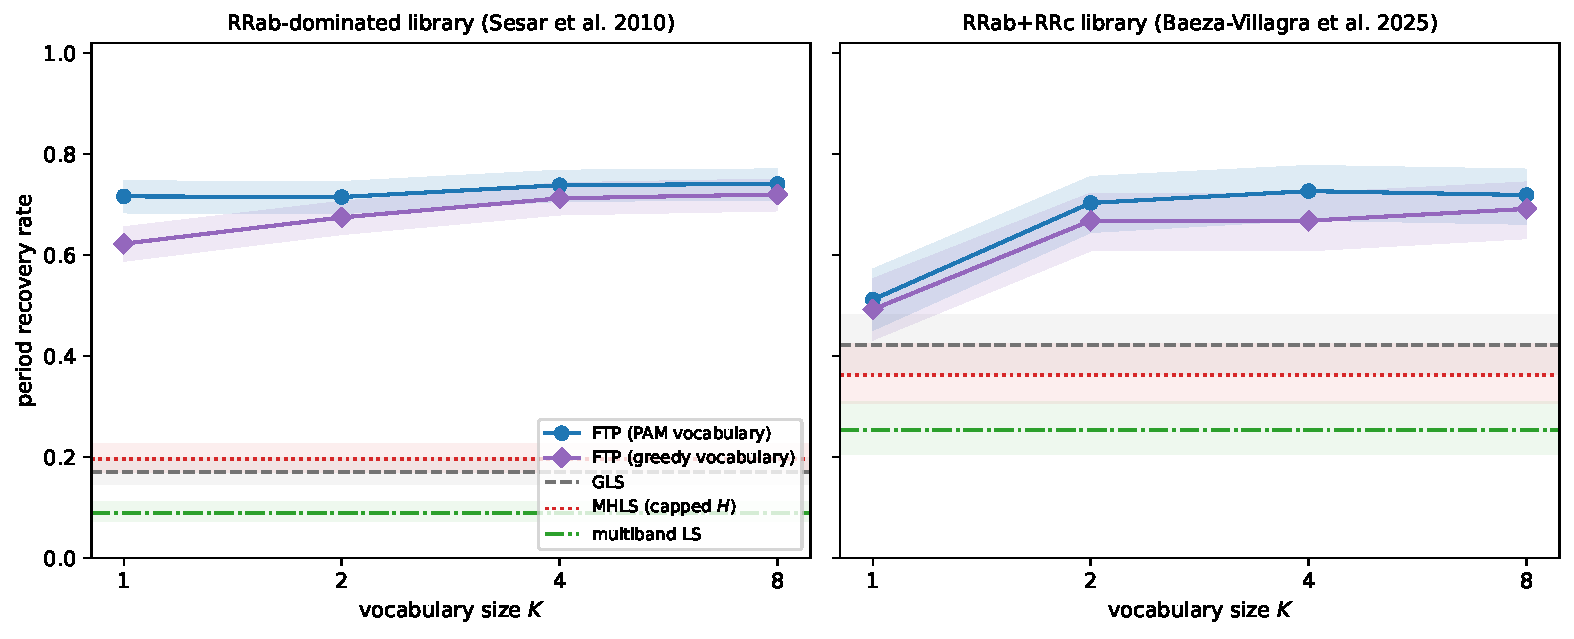
\includegraphics[width=\textwidth]{plots/recovery_vs_k_sparse.pdf}
    \caption{\label{fig:ksweep} Sparse-regime ($6$ epochs per band)
             period recovery versus vocabulary size $K$ for PAM and
             greedy vocabularies, with the $K$-independent baselines as
             reference bands.  \emph{Left}: the RRab-dominated
             \citet{Sesar_etal_2010} universe ($768$ pooled sources) is
             flat in $K$ -- a single well-chosen medoid already covers
             the population.  \emph{Right}: the morphologically diverse
             RRab$+$RRc universe of \citet{Baeza-Villagra_etal_2025}
             ($256$ sources) needs $K = 2$: the $K{=}1 \rightarrow 2$
             jump is $+0.19$ (McNemar $p \approx 8\times10^{-9}$),
             after which the curve is flat.}
\end{figure*}

Figure~\ref{fig:ksweep} asks how large the vocabulary must be, in the
regime where it matters (six epochs per band).  On the RRab-dominated
\citet{Sesar_etal_2010} universe the pooled PAM curve at
$K = 1, 2, 4, 8$ is $0.716$, $0.715$, $0.738$, $0.741$ with mutually
overlapping Wilson intervals; the paired $K{=}1$-versus-$K{=}2$
contrast is $34$ vs.\ $33$ discordant sources ($p = 1.0$) -- the curve
is flat in $K$ within the sampling noise, and the smallest $K$ whose
interval overlaps the best cell's is $K = 1$.  (A naive
$98\%$-of-maximum rule would return $K = 4$; the differences it chases
are not significant.)  On the RRab$+$RRc universe of
\citet{Baeza-Villagra_etal_2025} the same curve is $0.512$, $0.703$,
$0.727$, $0.719$: the $K{=}1 \rightarrow 2$ jump of $+0.191$ is highly
significant ($13$ vs.\ $62$ discordant, $p \approx 8\times10^{-9}$)
and the curve is flat thereafter.  The two panels together give the
honest reading: \emph{vocabulary size matters when the target
population is morphologically diverse} -- one medoid cannot serve both
RRab and RRc -- \emph{and is a second-order effect for a
shape-homogeneous class}, where the gain from $K = 1$ to $K = 8$ is at
most $\sim 0.03$ and statistically marginal.  Even at $K = 1$ every
FTP point sits far above the sparse-regime baselines (GLS $0.171$,
MHLS $0.197$, MBLS $0.090$ on the Sesar universe; GLS $0.422$ on the
diverse universe).  This recovery-rate flatness is complementary to
the significance cost of Section~\ref{sec:fap}, where enlarging $K$
raises the catalog-max detection threshold: together they argue for
the smallest $K$ that covers the class morphology.

\subsection{Robustness arms and empirical photometric errors}
\label{sec:simval-robust}

\begin{table}
\centering
\caption{\label{tab:robustness}
Robustness arms (single seed, $256$ sources per cell, $K = 2$,
$10^4$-frequency grid): period-recovery rate at $N = 4/8/12$ epochs per
band.  Holdout: truth shapes drawn from a held-out half of the
library, so the vocabulary never contains the generating shapes.
Cross-universe: truth from the RRab$+$RRc DECam universe, library
and vocabularies from the Sesar universe.  Band-amplitude: truth
amplitudes differ by a factor $1.4$ between $g$ and $r$, violating the
shared-amplitude model.}
\footnotesize
\begin{tabular}{llccc}
\hline\hline
Arm & Method & $N{=}4$ & $N{=}8$ & $N{=}12$ \\
\hline
holdout ($50\%$)  & FTP (PAM)    & $0.164$ & $0.891$ & $0.965$ \\
                  & FTP (greedy) & $0.152$ & $0.879$ & $0.973$ \\
                  & GLS          & $0.047$ & $0.449$ & $0.898$ \\
\hline
cross-universe    & FTP (PAM)    & $0.102$ & $0.695$ & $0.973$ \\
                  & FTP (greedy) & $0.109$ & $0.887$ & $0.988$ \\
                  & GLS          & $0.086$ & $0.672$ & $0.926$ \\
\hline
band-amp.\ $1.4$  & FTP (PAM)    & $0.082$ & $0.898$ & $0.988$ \\
                  & FTP (greedy) & $0.031$ & $0.793$ & $0.988$ \\
                  & GLS          & $0.047$ & $0.328$ & $0.867$ \\
\hline
\end{tabular}
\end{table}

Table~\ref{tab:robustness} stresses the three assumptions the headline
setup makes.  With half the library held out of vocabulary construction
(truth shapes never available as templates), the sparse-regime advantage
survives essentially intact ($0.891$ vs.\ $0.449$ at $N = 8$): the
vocabulary generalizes across shapes rather than memorizing them.  With
a $1.4\times$ band-amplitude ratio -- misspecifying the shared-amplitude
signal model -- the advantage again persists ($0.898$ vs.\ $0.328$ at
$N = 8$).  The cross-universe arm is the hardest test and the most
informative: with RRab$+$RRc truth but a Sesar-only library, the
\emph{unsupervised} PAM vocabulary degrades toward GLS ($0.695$ vs.\
$0.672$ at $N = 8$, and one source \emph{behind} GLS at $N = 16$,
$0.996$ vs.\ $1.000$), while the \emph{recovery-driven} greedy
vocabulary -- which sees a simulated population from the target
universe during selection -- adapts and retains the full advantage
($0.887$ at $N = 8$).  When the library may not span the target
population, the supervised selector is the safer choice.

A fourth arm replaces the synthetic noise model with the empirical ZTF
error-versus-magnitude relation measured from the real light curves
used for the cadence models of this paper's follow-up work; the
empirical curve is a factor $1.4$--$3.5$ larger than the synthetic one
over its measured range ($14.3 \leq m \leq 18.5$).  Recovery is
essentially unchanged -- FTP(PAM) $0.215/0.918/0.988$ at $N = 4/8/12$
versus $0.233/0.902/0.984$ pooled synthetic (this arm ran at $K = 4$;
the Sesar curve is flat in $K$) -- because RR\,Lyrae-scale amplitudes
keep the per-epoch shape signal-to-noise high: in this regime recovery
is limited by epoch count and the window function, not by photometric
noise.

\subsection{Cost versus accuracy}
\label{sec:simval-cost}

Finally, the same harness times the FTP against the non-linear
template-fitting procedure it replaces: a Sesar-style oracle
\citep[cf.][]{Sesar_etal_2010,Sesar_etal_2016} that, at every
(template, frequency) pair, brute-force scans $128$ phase shifts,
solves amplitude and per-band offsets linearly at each, and polishes
the best phase by golden-section refinement.  On a $32$-source
subsample at $1500$ frequencies with the $K = 2$ vocabulary the two
return \emph{identical} recovered periods (recovery $0.344$ for both)
-- consistent with the $<10^{-6}$ agreement of their per-frequency
optima -- at $23.5$\,s for the FTP versus $56.2$\,s for the oracle, a
measured ${\approx}2.4\times$ wall-time advantage under this harness's
deliberately modest settings ($128$ phase trials, $N_{\rm obs} \leq
120$).  The ratio is structural rather than incidental: the oracle's
per-frequency cost scales with the number of phase trials \emph{and}
with $N_{\rm obs}$, while the FTP's per-frequency cost is independent
of $N_{\rm obs}$ (Section~\ref{sec:compreqs}), so the advantage grows
without bound with denser phase grids and longer light curves --
the single-band measurements of Figure~\ref{fig:timingndata} reach
${\gtrsim}480\times$ by $N_{\rm obs} = 250$ against a generic
non-linear optimizer.  Reported end-to-end per-star costs of
survey template-fitting pipelines are larger by further orders of
magnitude, but those figures fold in denser phase grids, per-band
template sets, and infrastructure external to the fitting algorithm,
so we quote only the like-for-like in-harness ratio as a measured
result.

\section{Discussion}\label{sec:discussion}

Template fitting is a powerful technique for accurately recovering
the period and amplitude of objects with \emph{a priori} known
lightcurve shapes. It has been used in the literature by, e.g.
\cite{Stringer_et_al_2019,Sesar_etal_2016, Sesar_etal_2010}, to detect RR Lyrae in the
SDSS, PS1, and DES datasets, where it has been shown to produce purer
samples of RR Lyrae at a given completeness. The computational
cost of current template fitting algorithms, however, prevents their
application to larger datasets.

We have presented a novel template fitting algorithm that extends
the Lomb-Scargle periodogram \citep{Lomb_1976,Scargle_1982,Barning_1963,Vanicek_1971}
to handle non-sinusoidal signals that can be expressed in terms of
a fixed truncated Fourier series with a reasonably small number of harmonics
($H\lesssim 10$).

On its default scan path the fast template periodogram (FTP) asymptotically scales as
$\bigO(N_fH^2\log HN_f + N_fH^3)$ (including the extra factor of $H$ needed to resolve a peak),
while previous template fitting algorithms such as the one used in the \texttt{gatspy} library
\citep{gatspy} scale as $\bigO(N_fN_{\rm obs})$. The FTP's cost is set by computing the polynomial
coefficients and the per-frequency phase maximisation, and is independent of $N_{\rm obs}$; the
reference root-finding path instead carries an $N_fH^4$ term.
The remaining $H^3$ scaling restricts templates to those that are
sufficiently smooth to be explained by a small number of Fourier terms.

FTP also improves the accuracy of previous template fitting algorithms,
which rely on non-linear optimization at each trial frequency to minimize
the $V$ of the template fit. The FTP routinely finds superior fits over
non-linear optimization methods.

An open-source Python implementation of the FTP is available at
GitHub.\footnote{\url{https://github.com/PrincetonUniversity/FastTemplatePeriodogram}}
The current implementation could likely be improved by:

\begin{enumerate}
    \item Further optimising the polynomial coefficient assembly and the
          scan+polish maximisation---for example by moving the per-chunk
          assembly onto vectorised or compiled kernels---beyond the measured
          factor of ${\sim}25$--$35$ that the scan+polish default already gains
          over the reference root-finding path.
    \item Exploiting the embarassingly parallel nature of the FTP using GPU's.
    \item Extending the vocabulary search of
          Sections~\ref{sec:vocab}--\ref{sec:simval} -- which fits each
          template separately and reports the per-frequency maximum --
          to a \emph{joint} shared-frequency model with independent
          amplitudes and phases per template.  The polynomial-root
          formulation generalises to that setting analogously to the
          multi-band extension of Appendix~\ref{sec:shphmult}.
\end{enumerate}

For a constant baseline, the default implementation improves on full non-linear optimization by
more than two orders of magnitude ($\gtrsim 480\times$ measured by $N_{\rm obs}=250$) once the sampling
is well enough conditioned that the scan avoids its exact-root fallback, with the advantage growing as
$N_{\rm obs}$ increases. This work presents the mathematical shortcut that, realised through the
scan+polish maximiser, makes template fitting a fast and valuable tool for detecting non-sinusoidal
periodic signals of specified shape in large time-series datasets.

A real-survey demonstration of the multi-band FTP against
single-band Lomb--Scargle, multi-band Lomb--Scargle
\citep{Vanderplas+Ivezic_2015}, and full non-linear template fitting
\citep{Sesar_etal_2016} is the natural next step and is the subject of
follow-up work using the Zwicky Transient Facility public DR22 sparse
multi-band photometry of RR\,Lyrae, with the Gaia DR3 RR\,Lyrae catalogue \citep{Clementini_etal_2023} serving as an all-sky cross-matching benchmark.



%\begin{table}
%\centering
%\begin{tabular}{l|l|l|l}
%Survey     & $N_{\rm LC}$ & $N_{\rm obs}$ & Refs. \\
%\hline\hline
%CoRoT      & $1.5\times 10^5$  &  53,000       &       \\
%\hline
%Kepler     & $1.7\times 10^5$  &  65,000       &       \\
%\hline
%HATNet     & $5.6\times 10^6$  &  10,000       &       \\
%\hline
%Gaia       &           $10^9$  &  70           &       \\
%\hline
%SuperWASP  & $3.2\times 10^7$  &  13,870       &       \\
%\hline
%OGLE-IV    &           $10^9$  &  5000         &       \\
%\hline
%LSST       & $3.7\times 10^{10}$ &  825          &       \\
%\hline
%\end{tabular}
%\caption{\label{tab:surveypars} Survey parameters used for Figure \ref{fig:surveys}.
%\todo{Add references (if we decide to keep this figure)}}
%\end{table}

%\begin{figure}
%\centering
%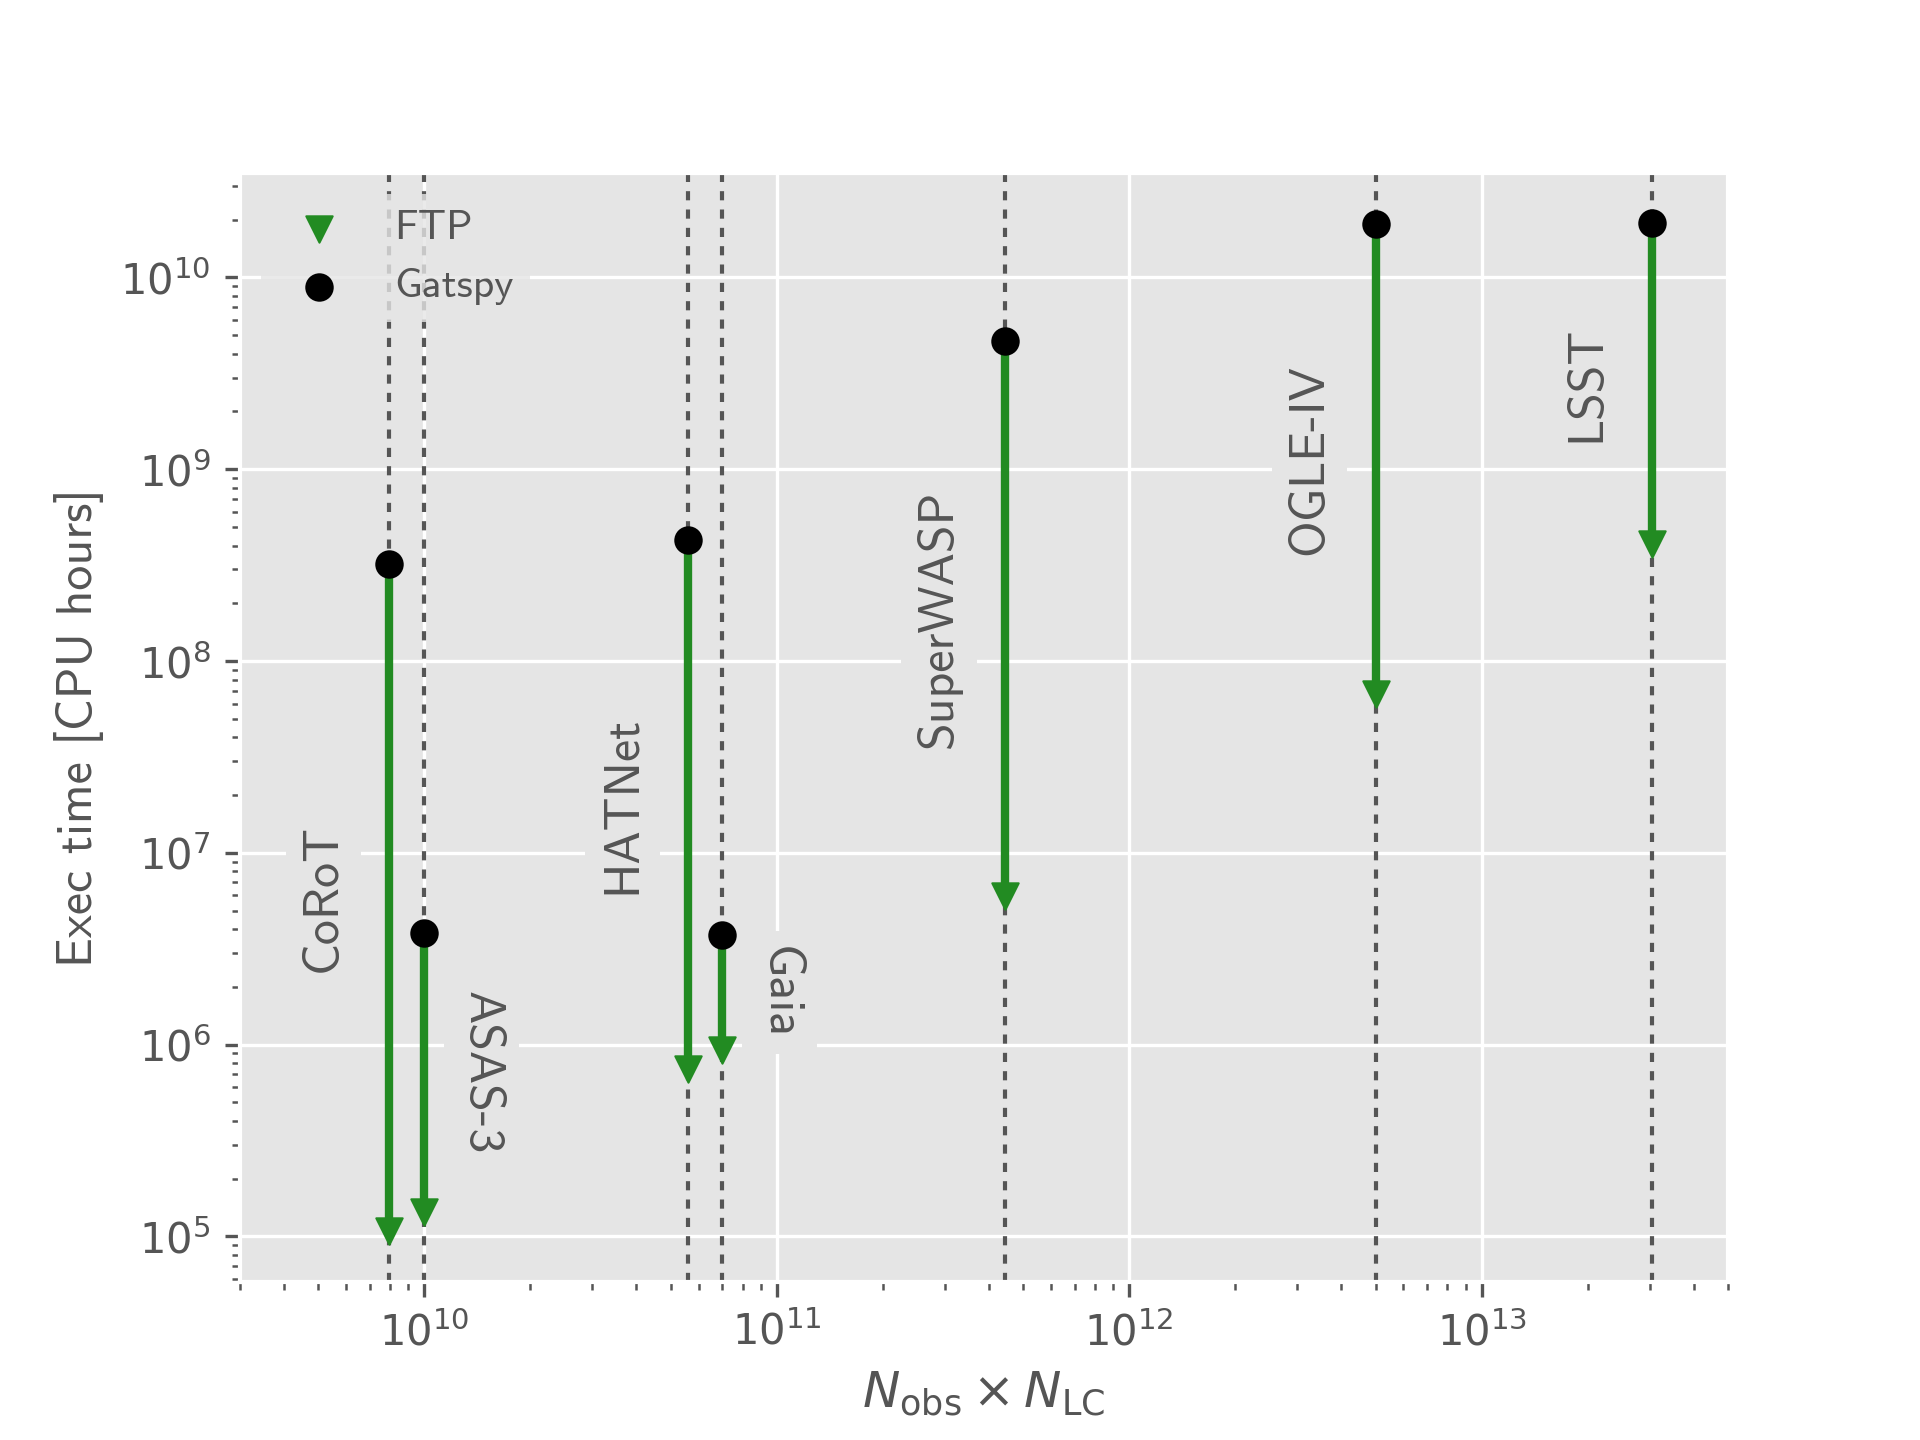
\includegraphics[width=0.5\textwidth]{plots/timing_for_various_surveys.png}
%%\caption{\label{fig:surveys} Computational resources needed for performing
%a single template periodogram ($H=6$) on an entire survey dataset. Our
%python implementation of FTP improves computational efficiency of template
%searches by orders of magnitude in most cases, and in one case by over
%three orders of magnitude (CoRoT). Parameters for $N_{\rm obs}$ and $N_{\rm LC}$
%were estimated from publicly available information (see text).}
%\end{figure}

%As pointed out in \cite{Vanderplas+Ivezic_2015}, current template fitting
%procedures are too slow to be practical for LSST-sized time-domain surveys.
%We attempt to quantify the improvement in computational efficiency for
%several important time-domain surveys, using estimated survey values for
%$N_{\rm obs}$, the number of observations per object, and $N_{\rm LC}$,
%the number of objects with lightcurves in the survey.

%Figure \ref{fig:surveys} shows estimated computation time for a single
%template periodogram performed on the entirety of a given survey. For all
%surveys, the FTP improves computational efficiency in one case over
%three orders of magnitude, but typically between 2-3 orders of magnitude.
%Improving the existing implementation, and porting to C/C++ and CUDA,
%should further improve these numbers.

%Template fitting remains prohibitvely slow for practical applications to
%large time-domain surveys, but this work presents a mathematical shortcut
%that could eventually make template fitting a fast and valuable tool.

%Appendix: Proof that GLS is recovered when H=1



\section*{Acknowledgements}
\begin{acknowledgements}
    Joel Hartman and GB acknowledge support from NASA grant NNX17AB61G. JTV is supported by the University of Washington eScience Institute, with funding from the Alfred P. Sloan Foundation, the Gordon and Betty Moore Foundation, and the Washington Research Foundation.
\end{acknowledgements}

\section*{Data availability}
The \texttt{ftperiodogram} code implementing the fast template
periodogram is openly available at
\url{https://github.com/PrincetonUniversity/FastTemplatePeriodogram}.
The manuscript sources, the figure-generation scripts, and the saved
results underlying every figure and table in this article are
available at
\url{https://github.com/PrincetonUniversity/FastTemplatePeriodogramPaper}.
The simulation-experiment artifacts -- per-run \texttt{results.json}
files with their full configuration blocks and random seeds -- are
versioned under \texttt{experiments/} in the code repository, so every
quoted number regenerates from a committed script and recorded seed.
The real Zwicky Transient Facility light curves used for the empirical
cadence and photometric-error models were retrieved from the public
IRSA ZTF light-curve service (\texttt{nph\_light\_curves}, DR22-era
release); the cached light curves, including per-record query
provenance and the observed MJD span, are stored alongside the
experiment code.

\bibliographystyle{apj}
\bibliography{refs}

\begin{appendix}

\section{Full derivation of the fast template periodogram}\label{app:fullderivation}

This appendix gives the explicit algebra summarised in
Section~\ref{sec:derivations}.  We present (i) the general form of
the gradient conditions for a weighted-least-squares periodogram;
(ii) the polynomial expansion of the phase-shifted template; (iii)
the closed-form solution to the linear least-squares sub-problem at
fixed phase shift $\theta_2$; (iv) the reduction of the residual sum
of squares $V$ to the compact periodogram form of
Equation~\ref{eq:Pofomega}; (v) the polynomial expansion of the
weighted statistics $MM$ and $YM$ in terms of $\eith = e^{i\theta_2}$
and the trigonometric sums of
Equations~\ref{eq:CCdef}--\ref{eq:YSdef}; and (vi) the algebraic
identity converting the non-linear condition
Equation~\ref{eq:theta2cond} into the polynomial root-finding
condition of Equation~\ref{eq:finalpoly}.

\subsection{General form of the gradient conditions}
\label{app:simpconds}

The optimality condition Equation~\ref{eq:chi2conds} can be written
explicitly for each parameter $\theta_j$ as follows.  Writing
$\hat{y}_i = \hat{y}(\omega t_i; \theta)$ and
$\partial_j\hat{y}_i = \left.\partial\hat{y}(\omega t;\theta)/\partial\theta_j\right|_{t=t_i}$,
\begin{equation}\label{eq:appsimpconds}
\begin{split}
0 &= \left.\frac{\partial V}{\partial\theta_j}\right|_{\theta=\theta_{\rm opt}}\\
  &= -2\sum_i \wgt_i\left(y_i - \hat{y}_i \right)(\partial_j\hat{y})_i, \\
\sum_i \wgt_iy_i(\partial_j\hat{y})_i &= \sum_i \wgt_i \hat{y}_i(\partial_j\hat{y})_i.
\end{split}
\end{equation}
This is a general result that extends to all least-squares
periodograms.  To simplify the derivations below we adopt the
weighted-average notation
\begin{eqnarray}
\savg{X} &\equiv& \sum_i \wgt_i X_i,\\
\savg{XY} &\equiv& \sum_i \wgt_i X_iY_i,\\
\scov(X, Y) &\equiv& \savg{XY} - \savg{X}\savg{Y},\\
\svar(X) &\equiv& \scov(X, X).
\end{eqnarray}

\subsection{Phase-shifted template expansion}
\label{app:shifttemplate}

The transposed template
$\Mshft = \mathbf{M}(\omega t - \theta_2)$ can be expressed as
\begin{align}
\Mshft(\omega t) &= \sum_n c_n\cos n\left(\omega t - \theta_2 \right) + s_n\sin{n\left(\omega t - \theta_2 \right)} \nonumber\\
                &= \sum_n\left(c_n\cos{n\theta_2}-s_n\sin{n \theta_2}\right)\cos{n\omega t} \nonumber \\
                &\qquad + \left(s_n\cos{n\theta_2} + c_n\sin{n \theta_2}\right)\sin{n\omega t} \nonumber\\
                &= \sum_n\left(\alpha_n \eith^n + \alpha_n^{*} \eith^{-n}\right)\cos{n\omega t} \nonumber \\
                &\qquad - i\left(\alpha_n \eith^n - \alpha_n^{*} \eith^{-n}\right)\sin{n\omega t} \nonumber\\
                &= \sum_n A_n(\eith)\cos{n\omega t} + B_n(\eith)\sin{n\omega t},
\end{align}
where $\alpha_n = (c_n + is_n)/2$ and $\eith\equiv e^{i\theta_2}$.
We also define the weighted statistics
\begin{align}
\YMhat &\equiv \savg{y\Mshft}, &
\MMhat &\equiv \savg{\Mshft^2}, \nonumber\\
\Mbar &\equiv \savg{\Mshft}, &
MM &\equiv \svar(\Mshft) = \MMhat - \Mbar^2, \nonumber\\
YM &\equiv \scov(\Mshft, y) = \YMhat - \bar{y}\Mbar.
\end{align}

\subsection{Closed-form linear least squares for $(\theta_1, \theta_3)$}
\label{app:closedform}

For a given phase shift $\theta_2$, the optimal amplitude and offset
are obtained by setting the partial derivatives of $V$ with respect
to $\theta_1$ and $\theta_3$ to zero:
\begin{align}
0 = \frac{\partial V}{\partial\theta_1} &= -2\sum_i \wgt_i(y_i - \theta_1\Mshft - \theta_3)\Mshft \nonumber \\
   &\propto \YMhat - \theta_1 \MMhat - \theta_3 \Mbar,\\
0 = \frac{\partial V}{\partial\theta_3} &= -2\sum_i \wgt_i(y_i - \theta_1\Mshft - \theta_3) \nonumber \\
   &\propto \bar{y} - \theta_1 \Mbar - \theta_3.
\end{align}
This $2\!\times\!2$ system can be written as
\begin{equation}
\begin{pmatrix} \MMhat & \Mbar \\ \Mbar & 1 \end{pmatrix}
\begin{pmatrix} \theta_1 \\ \theta_3 \end{pmatrix}
=
\begin{pmatrix} \YMhat \\ \bar{y}\end{pmatrix},
\end{equation}
with closed-form solution
\begin{equation}\label{eq:appthetaopt}
\begin{pmatrix} \theta_1 \\ \theta_3 \end{pmatrix}
=
\begin{pmatrix} YM / MM \\ \bar{y} - \Mbar\,(YM / MM)\end{pmatrix},
\end{equation}
where $MM = \MMhat - \Mbar^2$ and
$YM = \YMhat - \bar{y}\Mbar$.  The fitted model is then
\begin{equation}
\hat{y}_i = \bar{y} + \left(\frac{YM}{MM}\right)\!\left(M_i - \Mbar\right).
\end{equation}

\subsection{The periodogram in terms of $YY$, $YM$, and $MM$}
\label{app:periodogramform}

Substituting Equation~\ref{eq:appthetaopt} into $V$,
\begin{align}
V &= \sum_i \wgt_i (y_i - \hat{y}_i)^2 = \sum_i \wgt_i (y_i^2 - 2y_i\hat{y}_i + \hat{y}_i^2) \nonumber\\
  &= YY - 2\frac{(YM)^2}{MM} + \frac{(YM)^2}{MM} \nonumber\\
  &= YY - \frac{(YM)^2}{MM}.
\end{align}
Since $V_0 = YY$,
\begin{equation}
P(\omega) = 1 - \frac{V}{V_0} = \frac{(YM)^2}{YY\cdot MM},
\end{equation}
which is Equation~\ref{eq:Pofomega} of the body.

\subsection{Polynomial expansion of $MM$ and $YM$}
\label{app:mmandym}

The autocovariance of the template values, $MM$, is given by
\begin{align}
MM &\equiv \sum_i \wgt_i M_i^2 - \left(\sum_i \wgt_i M_i\right)^2 \nonumber\\
   &= \sum_i \wgt_i \left(\sum_n A_n\cos{\omega n t_i} + B_n\sin{\omega n t_i}\right)^2 \nonumber\\
   &\qquad - \left(\sum_n A_n C_n + B_n S_n\right)^2 \nonumber\\
   &= \sum_{n,m} A_n A_m CC_{nm} + 2 A_n B_m CS_{nm} \nonumber\\
   &\qquad + B_n B_m SS_{nm},
\end{align}
using the symmetry
$\sum_{n,m} A_n B_m CS_{nm} = \sum_{n,m} A_m B_n CS_{mn}$.

The products $A_n A_m$, $A_n B_m$, $B_n B_m$ expand as
\begin{align}
A_n A_m &= \alpha_n\alpha_m \eith^{n+m} + \alpha^{*}_n\alpha_m \eith^{m-n} \nonumber\\
        &\qquad + \alpha_n\alpha^{*}_m \eith^{n-m} + \alpha^{*}_n\alpha^{*}_m \eith^{-n-m},\\
A_n B_m &= -i\bigl[\alpha_n\alpha_m \eith^{n+m} + \alpha^{*}_n\alpha_m \eith^{m-n} \nonumber\\
        &\qquad - \alpha_n\alpha^{*}_m \eith^{n-m} - \alpha^{*}_n\alpha^{*}_m \eith^{-n-m}\bigr],\\
B_n B_m &= -\bigl[\alpha_n\alpha_m \eith^{n+m} - \alpha^{*}_n\alpha_m \eith^{m-n} \nonumber\\
        &\qquad - \alpha_n\alpha^{*}_m \eith^{n-m} + \alpha^{*}_n\alpha^{*}_m \eith^{-n-m}\bigr].
\end{align}

Substituting these into the $MM$ sum gives the polynomial form
\begin{align}\label{eq:appMM}
MM_{nm} &= A_n A_m CC_{nm} + 2 A_n B_m CS_{nm} + B_n B_m SS_{nm} \nonumber\\
        &= \alpha_n\alpha_m\CCt_{nm}\eith^{n+m} + 2\alpha_n\alpha^{*}_m\CSt_{nm}\eith^{n-m} \nonumber\\
        &\qquad + \alpha^{*}_n\alpha^{*}_m\SSt_{nm}\eith^{-(n+m)},
\end{align}
where
\begin{align}
\CCt_{nm}  &= (CC_{nm} - SS_{nm}) - i\left(CS + CS^T\right)_{nm}, \\
\CSt_{nm}  &= (CC_{nm} + SS_{nm}) + i\left(CS - CS^T\right)_{nm},\\
\SSt_{nm}  &= (CC_{nm} - SS_{nm}) + i\left(CS + CS^T\right)_{nm}.
\end{align}

Analogously, the cross term $YM$ expands as
\begin{align}\label{eq:appYM}
YM_{k} &= A_k YC_k + B_k YS_k \nonumber\\
       &= \alpha_k YC_k\eith^k + \alpha_k^{*} YC_k\eith^{-k} \nonumber\\
       &\qquad - i\left(\alpha_k YS_k\eith^k - \alpha^{*}_k YS_k\eith^{-k}\right) \nonumber\\
       &= \alpha_k\YCt_k \eith^k + \alpha^{*}_k\YCt_k^{*} \eith^{-k},
\end{align}
where $\YCt_k \equiv YC_k - i YS_k$.

\subsection{From the non-linear condition to the polynomial form}
\label{app:polynomialform}

The non-linear condition Equation~\ref{eq:theta2cond} can be
rewritten in terms of the rescaled quantities
$YM' \equiv \eith^H YM$ and $MM' \equiv \eith^{2H} MM$, which (from
Equations~\ref{eq:appMM}--\ref{eq:appYM}) are polynomials in $\eith$
of degree $2H$ and $4H$, respectively.  Their derivatives are
\begin{align}
\partial YM' &= H\eith^{H-1} YM + \eith^H \partial YM,\\
\partial MM' &= 2H\eith^{2H-1} MM + \eith^{2H}\partial MM.
\end{align}
Combining these,
\begin{align}\label{eq:appfinalpoly}
0 &= 2 MM\,\partial(YM) - YM\,\partial(MM) \nonumber\\
  &= \eith^{3H+1}\bigl[2 MM\,\partial(YM) - YM\,\partial(MM)\bigr] \nonumber\\
  &= 2\,\eith^{2H} MM\bigl[\eith^{H+1}\partial(YM)\bigr] \nonumber\\
  &\qquad - \eith^H YM\bigl[\eith^{2H+1}\partial(MM)\bigr] \nonumber\\
  &= 2\, MM'\bigl[\eith\,\partial(YM') - H\,(YM')\bigr] \nonumber\\
  &\qquad - YM'\bigl[\eith\,\partial(MM') - 2H\,(MM')\bigr] \nonumber\\
  &= \eith\bigl[2\, MM'\,\partial(YM') - YM'\,\partial(MM')\bigr] \nonumber\\
  &\qquad - 2H\bigl[MM'\,YM' - YM'\,MM'\bigr] \nonumber\\
  &= 2\, MM'\,\partial(YM') - YM'\,\partial(MM').
\end{align}
The last step assumes $\eith\ne 0$, which holds since
$\eith = e^{i\theta_2}$ lies on the unit circle for all real
$\theta_2$.  Equation~\ref{eq:appfinalpoly} is the polynomial
root-finding condition of Equation~\ref{eq:finalpoly} in the body.
Although the nominal degree of Equation~\ref{eq:appfinalpoly} is
$6H-1$ ($\deg MM' = 4H$, $\deg \partial(YM') = 2H-1$), the
degree-$(6H{-}1)$ terms cancel identically: writing $ym$ and $mm$ for
the leading coefficients of $YM'$ and $MM'$, the leading coefficient
of $2\,MM'\,\partial(YM')$ is $2\,(2H)\,mm\,ym$ and that of
$YM'\,\partial(MM')$ is $(4H)\,ym\,mm$ (a consequence of
$\deg MM' = 2 \deg YM'$), so the true degree is at most $6H-2$.

\section{Multi-band template periodograms and the sharing hierarchy}\label{sec:shphmult}

The single-band template periodogram extends to observations in $K$ filters ($N_k$ observations in the $k$-th filter, the $i$-th of which is denoted $\yk_i$) as a family of models that differ in which of the template's amplitude, phase, and offset are held common across the bands. We fit a periodic, multi-band template $\Mt = (\Mtk[1], \Mtk[2], ..., \Mtk[K]): [0, 2\pi)\rightarrow \mathbb{R}^K$ to all observations, and label the members of the resulting \emph{sharing hierarchy} by their names in the accompanying implementation (Table~\ref{tab:sharingmodes}). Freeing more parameters per band increases the model's flexibility at the price of a larger per-frequency solve. The three modes that retain a per-band offset (\texttt{independent}, \texttt{shared\_phase}, \texttt{floating\_offsets}) measure signal power against the per-band-centred variance $\sum_k \Wtk YY^{(k)}$, whereas the fully shared \texttt{sesar} model centres on the global mean; every member reduces to the single-band periodogram of Appendix~\ref{app:fullderivation} at $K=1$. The multi-band experiments in this paper use \texttt{floating\_offsets} (shared amplitude and phase, per-band free offset), the default mode, which we derive in Section~\ref{app:floatingoffsets} after the fully shared model.

\begin{table*}
\centering
\caption{\label{tab:sharingmodes}
Members of the multi-band sharing hierarchy, labelled by their name in the
accompanying implementation. Each mode fixes some of the template's
amplitude ($\theta_1$), phase ($\theta_2$), and offset ($\theta_3$) across
the $K$ bands and frees the rest per band. $V_0$ is the reference variance
that normalises the power (Equation~\ref{eq:Pofomega}); $\Wtk = \sum_i \wk_i$
is the fraction of the total inverse-variance weight in band $k$
($\sum_k \Wtk = 1$), and $\ybar$ is the global weighted mean (computed on the $\lk$-subtracted data for \texttt{sesar}). The final
column is the per-frequency cost of the phase maximisation, on top of the
$\bigO(KN_fH\log N_fH)$ NFFT summations that are common to every mode ($H$
is the harmonic order). All modes coincide with the single-band periodogram
at $K=1$.}
\footnotesize
\begin{tabular}{lllll}
\hline\hline
Mode (\texttt{code}) & Shared across bands & Free per band & Reference variance $V_0$ & Root cost / frequency \\
\hline
\texttt{independent}                    & (nothing)                                  & $\theta_1,\theta_2,\theta_3$ & $\sum_k \Wtk\, YY^{(k)}$          & $\bigO(KH^3)$ \\
\texttt{shared\_phase}                  & $\theta_2$                                 & $\theta_1,\theta_3$          & $\sum_k \Wtk\, YY^{(k)}$          & $\bigO((HK)^3)$ \\
\texttt{floating\_offsets}$^{\dagger}$  & $\theta_1,\theta_2$                        & $\theta_3$                   & $\sum_k \Wtk\, YY^{(k)}$          & $\bigO(H^3)$ \\
\texttt{sesar}                          & $\theta_1,\theta_2,\theta_3$ (fixed $\lk$) & ---                          & $\sum_{k,i}\wk_i(\yk_i-\lk-\ybar)^2$  & $\bigO(H^3)$ \\
\hline
\end{tabular}
\\[3pt]
{\raggedright\footnotesize $^{\dagger}$ Default mode used for the multi-band
experiments in this paper. \texttt{independent} is the per-band template
analogue of the \cite{Vanderplas+Ivezic_2015} multi-band periodogram;
\texttt{sesar} is the model of \cite{Sesar_etal_2016}.\par}
\end{table*}

\subsection{The fully shared model (\texttt{sesar})}
\label{app:sesarmode}

In the model of \cite{Sesar_etal_2016} the amplitude, phase, and offset are all shared across the bands, up to a fixed, known per-band offset $\lk$:

\begin{equation}
\yhk(t;\theta) = \theta_1\Mtk(\omega t - \theta_2) + \theta_3 + \lk
\end{equation}

where $\lk$ is a fixed relative offset for band $k$. The $V$ for this model is

\begin{equation}
V = \sum_{k=1}^{K}\sum_{i=1}^{N_k}\wk_i \left(\yk_i - \yhk_i\right)^2
\end{equation}

To make things simpler, we can set the $\lk$ values to 0 simply by subtracting them off from our observations; this means we take all $\yk_i \rightarrow \yk_i - \lk$. We have that

\begin{equation}
V = \sum_{k=1}^K \Wtk V_k
\end{equation}

Where $\Wtk \equiv \sum_{i=1}^{N_k}\wk_i$ and $\sum_{k=1}^K\Wtk = 1$. This means that the system of equations reduces to:

\begin{equation}
0 = \frac{\partial V}{\partial\theta_1} = \sum_{k=1}^K \Wtk\left(\YMh - \theta_1\MMh - \theta_3\Mbk\right)
\end{equation}

for the $\theta_1$ parameter, where $\YMh$, $\MMh$, $\Mbk$ are values from the single band case computed for each band individually, holding $\Wtk = 1$ for each band. That is:

%\begin{equation}
\begin{align}
\YMh &\equiv \frac{1}{\Wtk}\sum_{i=1}^{N_k}\wk_i \yk_i \Mtshftk(\omega t_i)\\
\MMh &\equiv \frac{1}{\Wtk}\sum_{i=1}^{N_k}\wk_i \left(\Mtshftk(\omega t_i)\right)^2\\
\Mbk &\equiv \frac{1}{\Wtk}\sum_{i=1}^{N_k}\wk_i \Mtshftk(\omega t_i)
\end{align}
%\end{equation}

For the offset $\theta_3$, we have

\begin{equation}
0 = \frac{\partial V}{\partial\theta_3} = \sum_{k=1}^K \Wtk\left(\yb - \theta_1\Mbk - \theta_3\right)
\end{equation}

Where $\yb$ is the weighted-mean for the $k$-th band ($\yb \equiv (1/\Wtk)\sum_{i=1}^{N_k}\wk_i\yk_i$), again with $\yk_i \rightarrow \yk_i - \lk$.

So if we redefine the quantities $\YMhat$, $\MMhat$, $\Mbar$, and $\bar{y}$ as weighted averages across the bands, i.e. $\YMhat = \sum_{k=1}^K \Wtk \YMh$, etc., the solution for the optimal parameters has the same form:

%\begin{equation}
\begin{align}
\theta_1 &= \left(\frac{YM}{MM}\right)\\
\theta_3 &= \bar{y} - \Mbar\left(\frac{YM}{MM}\right)
\end{align}
%\end{equation}

which means that the model for the $k$-th band is

\begin{equation}
\yhk = \bar{y} + \left(\frac{YM}{MM}\right)\left(M^{(k)}_i - \Mbar\right)
\end{equation}

The form of the periodogram has the same form as the single-band case:

%\begin{equation}
\begin{align}
V &=\sum_{k=1}^{K}\sum_{i=1}^{N_k}\wk_i \left(\yk_i - \yhk_i\right)^2\\
       &=\sum_{k=1}^{K}\sum_{i=1}^{N_k}\wk_i \left((\yk_i - \bar{y}) - \left(\frac{YM}{MM}\right)(M_i^{(k)} - \Mbar)\right)^2\\
       &=\sum_{k=1}^{K}\sum_{i=1}^{N_k}\wk_i \left((\yk_i - \bar{y})^2 - 2\left(\frac{YM}{MM}\right)(M_i^{(k)} - \Mbar)(\yk_i - \bar{y}) + \left(\frac{YM}{MM}\right)^2(M_i^{(k)} - \Mbar)^2\right)^2\\
       &=YY - 2\frac{(YM)^2}{MM} + \frac{(YM)^2}{MM}\\
       &=YY - \frac{(YM)^2}{MM}.
\end{align}
%\end{equation}

Since there is a single shared offset between the bands (i.e. we assume the mean magnitude is the same in all bands after subtracting $\lk$), the variance for the signal, $YY$, is not $\sum_{k=1}^{K}\sum_{i=1}^{N_k}\wk_i (\yk_i - \yb)^2$ but $\sum_{k=1}^{K}\sum_{i=1}^{N_k}\wk_i (\yk_i - \bar{y})^2$.

Construction of the polynomial for the multi-band case can be performed by first computing the polynomial expression for $\eith^{2H}\MMhat = \sum_{k=1}^{K}\sum_{i=1}^{N_k}\wk_i \left(\eith^{H}\Mk_i\right)^2$ and a separate polynomial expression for $\psi^H\Mbar$, which can then be squared and subtracted from $\psi^{2H}\MMhat$ to find $MM' = \eith^{2H}MM$.

For $YM' = \eith^H YM$, we merely compute $\eith^H\YMhat^{(k)}$ for each band, take the weighted average of the polynomial coefficients for all bands ($\eith^H\YMhat = \sum_k^K \Wtk \eith^H\YMhat^{(k)}$) and subtract the $\eith^H\bar{y}\Mbar$ polynomial to get $YM'$.

After computing the polynomials $MM'$ and $YM'$, the polynomial in Equation \ref{eq:finalpoly} can be computed quickly and the following steps for finding the optimal model parameters is the same as in the single band case.

\subsection{Floating per-band offsets (\texttt{floating\_offsets})}
\label{app:floatingoffsets}

The mode used for all of the multi-band experiments in this paper keeps the shared amplitude $\theta_1$ and phase $\theta_2$ of the \texttt{sesar} model but lets each band carry its own free offset $\theta_3^{(k)}$:
\begin{equation}
\yhk(t;\theta) = \theta_1\Mtk(\omega t - \theta_2) + \theta_3^{(k)}.
\end{equation}
Writing $V = \sum_k \Wtk V_k$ as before, the offset stationarity condition now acts on each band \emph{separately},
\begin{equation}
0 = \frac{1}{\Wtk}\frac{\partial V}{\partial\theta_3^{(k)}} = \yb - \theta_1\Mbk - \theta_3^{(k)},
\end{equation}
so the optimal offset $\theta_3^{(k)} = \yb - \theta_1\Mbk$ centres band $k$ on its \emph{own} weighted mean $\yb$. Substituting back, band $k$'s contribution is exactly the single-band, self-centred residual, and $V$ separates into a weighted average of single-band forms,
\begin{equation}
V = \sum_{k=1}^K \Wtk\left(YY^{(k)} - 2\theta_1\,YM^{(k)} + \theta_1^2\,MM^{(k)}\right) = \bandavg{YY} - 2\theta_1\,\bandavg{YM} + \theta_1^2\,\bandavg{MM},
\end{equation}
where $YM^{(k)} \equiv \YMh - \yb\,\Mbk$ and $MM^{(k)} \equiv \MMh - \bigl(\Mbk\bigr)^2$ are the \emph{centred} single-band moments $YM$ and $MM$ of Appendix~\ref{app:fullderivation} evaluated within band $k$---that is, computed about that band's own weighted mean, the same per-band objects that appear in Section~\ref{app:sharedphase}---$YY^{(k)}$ is the corresponding per-band-centred variance, and the band-combined quantities, written with an overline, are the \emph{plain} $\Wtk$-weighted band averages
\begin{equation}
\label{eq:foaverage}
\bandavg{YM} = \sum_{k=1}^K \Wtk\,YM^{(k)}, \qquad \bandavg{MM} = \sum_{k=1}^K \Wtk\,MM^{(k)}, \qquad \bandavg{YY} = \sum_{k=1}^K \Wtk\,YY^{(k)}.
\end{equation}
(The hat remains reserved for the \emph{uncentred} per-band moments $\YMh$, $\MMh$ of Section~\ref{app:sesarmode}, and the prime for the $\eith$-rescaled polynomials of Appendix~\ref{app:fullderivation}, e.g.\ $\bandavg{YM}{}' = \eith^{H}\,\bandavg{YM}$.) Because every band is already centred on its own mean, no global re-centring is required---unlike the \texttt{sesar} model (Section~\ref{app:sesarmode}), whose single shared offset forces the between-band $\bar{y}\Mbar$ and $\Mbar^2$ corrections. Minimising over the shared amplitude gives $\theta_1 = \bandavg{YM}/\bandavg{MM}$ and
\begin{equation}
P(\omega) = 1 - \frac{V}{\bandavg{YY}} = \frac{\bigl(\bandavg{YM}\bigr)^2}{\bandavg{YY}\;\bandavg{MM}},
\end{equation}
the single-band closed form of Equation~\ref{eq:Pofomega} with the band-averaged quantities in place of $YM$, $MM$, and $YY$. Since band averaging is linear in the per-band coefficient vectors, the rescaled polynomials $\bandavg{YM}{}' = \eith^{H}\,\bandavg{YM}$ and $\bandavg{MM}{}' = \eith^{2H}\,\bandavg{MM}$ have the same degrees ($2H$ and $4H$) as their single-band counterparts, so the maximisation over $\theta_2$ uses the identical degree-$(6H-2)$ root condition of Equation~\ref{eq:appfinalpoly}. Floating per-band offsets therefore cost essentially one single-band solve per frequency, independent of $K$ beyond the summations; at $K=1$ ($\Wtk=1$, $\yb=\ybar$) the mode collapses to the single-band periodogram.

\subsection{Shared phase, per-band amplitude (\texttt{shared\_phase})}
\label{app:sharedphase}

Relaxing the shared amplitude of \texttt{floating\_offsets} yields the \texttt{shared\_phase} model: a single phase $\theta_2$ is common to all bands, but each band fits its own amplitude and offset. For a fixed shared phase every band fits independently, so the variance explained is a sum of the per-band single-band contributions,
\begin{equation}
F(\eith) = \sum_{k=1}^K \Wtk\,\frac{\left(YM^{(k)}(\eith)\right)^2}{MM^{(k)}(\eith)},
\end{equation}
and the power is $P(\omega) = \max_{\theta_2} F(\eith)/\bandavg{YY}$, normalised by the same per-band-centred variance $\bandavg{YY} = \sum_k \Wtk YY^{(k)}$ (Equation~\ref{eq:foaverage}) as \texttt{floating\_offsets}.
The per-band amplitudes no longer collapse into a single band-combined polynomial. Clearing the common denominator $\prod_l\left(MM^{(l)}\right)^2$ (positive on the unit circle) gives the stationarity polynomial
\begin{equation}
G(\eith) = \sum_{k=1}^K \Wtk\, YM^{(k)}\, q_k \prod_{l\ne k}\left(MM^{(l)}\right)^2 = 0, \qquad q_k = 2\,MM^{(k)}\partial YM^{(k)} - \partial MM^{(k)}\,YM^{(k)},
\end{equation}
whose degree is at most $8HK-2$: each term's nominal leading coefficient at degree $8HK-1$ cancels identically, by the same top-term identity that reduces the single-band $q_k$. Its roots must be found explicitly, at a cost of $\bigO((HK)^3)$ per frequency. \texttt{shared\_phase} is thus the only member of the hierarchy whose phase maximisation \emph{couples} the bands into a single polynomial of $K$-dependent degree, making its per-frequency cost superlinear in $K$; the \texttt{independent} mode's $\bigO(KH^3)$ cost (Table~\ref{tab:sharingmodes}) is instead just $K$ repetitions of the single-band solve. Because the shared phase couples the bands, the per-band amplitudes cannot each be independently forced non-negative; this mode returns the power-maximising shared phase and its fitted per-band amplitudes.

\subsection{Computational cost across the hierarchy}
\label{app:mbcost}

For every mode the per-band NFFT summations cost $\bigO(KN_fH\log N_fH)$ over the full frequency grid, independent of the sharing mode. The per-frequency phase maximisation is where the modes differ. The coupled-but-cheap members \texttt{floating\_offsets} and \texttt{sesar} each assemble a single band-combined polynomial of degree at most $6H-2$ (Equation~\ref{eq:foaverage} and the \texttt{sesar} construction of Section~\ref{app:sesarmode}) and solve it at the single-band cost $\bigO(H^3)$ per frequency, so their total cost $\bigO(KN_fH\log N_fH + N_fH^3)$ exceeds a single-band periodogram's only through the $K$-fold NFFT summations; \texttt{independent} runs $K$ such solves, at $\bigO(KN_fH^3)$. Only \texttt{shared\_phase} is genuinely more expensive: its degree-$(8HK-2)$ stationarity polynomial $G$ costs $\bigO((HK)^3)$ per frequency. The implementation accompanying this paper replaces that root-finding with a direct scan of $F(\eith)$ on $\bigO(HK)$ trial phases, forming and solving $G$ only at those frequencies where \emph{some} band's template-variance polynomial $|MM^{(k)}|$ nearly vanishes on the unit circle (its minimum over the circle falling below a fixed fraction of its maximum). This removes the $\bigO((HK)^3)$ cost away from such deep-$|MM|$ dips, but not at them, where the exact root path is still run and the better of the two solutions kept, so the saving is opportunistic rather than guaranteed. The realised speedup is therefore strongly configuration-dependent: on well-conditioned dense-grid \texttt{shared\_phase} data ($K=2$) we measure the scan to be $1.3\times$ faster than the reference root path at $H=3$ and $5.4\times$ at $H=8$, but on sparse or otherwise deep-$|MM|$ sampling, where the fallback fires at most frequencies, the cost approaches that of the reference and the speedup collapses toward $1\times$. Since the polynomial step dominates in most applications, the multi-band template periodogram in the shared-amplitude modes is not significantly more computationally intensive than the single-band case.

\section{Alias breakdown of the simulated recovery rates}
\label{app:aliases}

The headline recovery criterion of Section~\ref{sec:simval} --
$|P_{\rm rec}-P_{\rm true}|/P_{\rm true} < 0.01$, exact only -- has one
known blind spot on this search band: a $\pm1$\,yr$^{-1}$ window beat
displaces the frequency by only $|\Delta f| = 1/365.25$\,cyc\,day$^{-1}$,
a fractional period error of at most $0.27\%$ for $f \geq
1$\,cyc\,day$^{-1}$, so the fractional criterion cannot distinguish a
year beat from an exact recovery.  Every scored (method, cell) pair
therefore persists its per-source recovered periods, and
Table~\ref{tab:aliases} re-scores them under baseline-aware phase
coherence, $|\Delta f|\,T < 0.5$ \citep[the accumulated-phase-drift
convention of][]{Graham_etal_2013}: over the $T = 1095.75$\,d baseline a
year beat accumulates $|\Delta f|\,T = 3$ cycles of drift and is cleanly
separated, while each non-exact recovery is assigned to the nearest
member of a named alias set (harmonic multiples $P/2$, $2P$, $3P$ and
the $\pm1$\,day$^{-1}$, $\pm1$\,yr$^{-1}$ window beats).

Three facts emerge.  First, the headline is safe: year-beat
contamination is at most one source per cell (and $\pm1$\,day$^{-1}$
beats are entirely absent at $N \geq 8$), and the two scoring
conventions agree on the headline rates -- e.g.\ FTP (PAM) at $N = 8$
is $689/768 = 0.897$ phase-coherent-exact versus $0.902$ under the
fractional criterion.  Second, the FTP's sparse-regime failures are
genuine misses, not aliases: at $N = 8$ none of its $79$ failures land
on a named alias.  Third, the MHLS plateau of
Figure~\ref{fig:nsweep} is harmonic aliasing, not noise: at $N = 40$
its $2P$ and $3P$ aliases account for $99/768$ sources, and crediting
them would lift MHLS from $0.868$ to $0.997$ -- the free-shape fit
detects \emph{a} periodicity but, lacking a shape prior, often locks
onto a harmonic of the fundamental.  The conditional-entropy statistic
shows the same signature at lower amplitude.  The full breakdown over
all epoch counts regenerates from the committed per-source artifacts
and scripts (see Data Availability).

\begin{table}
\centering
\caption{\label{tab:aliases}
Alias-resolved re-scoring of the pooled \citet{Sesar_etal_2010}-universe
recovery results ($768$ sources per cell, $K = 2$) under phase coherence
$|\Delta f|\,T < 0.5$.  Counts per cell: exact recoveries, harmonic
aliases, $\pm1$\,yr$^{-1}$ window beats, and misses.  ($P/3$ and
$\pm1$\,day$^{-1}$ entries are zero in every cell shown and are
omitted.)}
\footnotesize
\begin{tabular}{llrrrrrr}
\hline\hline
$N$ & Method & exact & $P/2$ & $2P$ & $3P$ & yr beat & miss \\
\hline
 8 & FTP (PAM)    & 689 & 0 & 0  & 0  & 0 & 79  \\
 8 & FTP (greedy) & 666 & 0 & 0  & 0  & 1 & 101 \\
 8 & GLS          & 307 & 0 & 1  & 0  & 1 & 459 \\
 8 & MHLS         & 428 & 0 & 15 & 6  & 1 & 318 \\
 8 & MBLS         & 184 & 1 & 0  & 0  & 0 & 583 \\
 8 & CE           &  60 & 1 & 13 & 3  & 0 & 691 \\
\hline
16 & FTP (PAM)    & 768 & 0 & 0  & 0  & 0 & 0   \\
16 & FTP (greedy) & 766 & 0 & 0  & 0  & 0 & 2   \\
16 & GLS          & 763 & 0 & 0  & 0  & 0 & 5   \\
16 & MHLS         & 595 & 0 & 70 & 23 & 1 & 79  \\
16 & MBLS         & 739 & 0 & 0  & 0  & 0 & 29  \\
16 & CE           & 643 & 1 & 39 & 1  & 0 & 84  \\
\hline
40 & FTP (PAM)    & 768 & 0 & 0  & 0  & 0 & 0   \\
40 & FTP (greedy) & 768 & 0 & 0  & 0  & 0 & 0   \\
40 & GLS          & 768 & 0 & 0  & 0  & 0 & 0   \\
40 & MHLS         & 667 & 0 & 83 & 16 & 0 & 2   \\
40 & MBLS         & 768 & 0 & 0  & 0  & 0 & 0   \\
40 & CE           & 762 & 0 & 6  & 0  & 0 & 0   \\
\hline
\end{tabular}
\end{table}

\end{appendix}

\end{document}
